\documentclass[12pt]{article}
\usepackage[utf8]{inputenc}
\usepackage[T1]{fontenc}
\usepackage{amsmath,amssymb}
\usepackage[margin=2.5cm]{geometry}
\usepackage{xcolor}
\usepackage{enumitem}
\usepackage{booktabs}
\usepackage{algpseudocode}
\usepackage{tikz}
\usetikzlibrary{arrows.meta,positioning,fit,decorations.pathreplacing}

%\usepackage{polski}
%\usepackage{todonotes}

\setlength{\parindent}{0pt}
\setlength{\parskip}{4pt}
\setlist{itemsep=1pt,topsep=2pt}

% Reviewer text italic, our text upright. Green: still open.
\newcommand{\upd}[1]{\textcolor{green!50!black}{#1}}
% reviewer comment (italic, emphasis bold italic); the argument is an internal label and is not printed
\newenvironment{rc}[1]{\par\medskip\noindent\itshape\renewcommand{\emph}[1]{\textbf{##1}}\ignorespaces}{\par}
\newenvironment{lead}{\par\medskip\noindent\itshape\renewcommand{\emph}[1]{\textbf{##1}}\ignorespaces}{\par}
\newcommand{\resp}{\par\smallskip\noindent\upd{[The answer to this point will be completed after the repeated experiments.]}\par\medskip}
\newcommand{\answer}[1]{\par\smallskip\noindent #1\par}
% change in the manuscript: where, previous text (not printed), revised text
\newcommand{\change}[3]{\par\smallskip\noindent\textbf{Revised text (#1).}\par
  {\leftskip=1.5em\noindent#3\par}}
\newcommand{\pending}[1]{\par\smallskip\noindent\upd{[This answer will be updated with the results of the repeated experiments.]}\par}
\newcommand{\todo}[1]{\upd{[#1]}}
\newcommand{\Cmax}{C_{\max}}

\begin{document}

\begin{center}
{\bf Answers to the Reviewer \#1 remarks\\[2mm]
``Quantum and Classical Annealing for Very Large-Scale Neighborhood Search in the Permutation Flow Shop Problem''}\\
BPASTS-05673-2026-02\\[5mm]
\end{center}

We thank both reviewers for reading the manuscript carefully and for their detailed comments. We agree with all of them and have revised the manuscript to address each point.

The revised manuscript separates the neighborhood, the selection model and the solver, gives a lemma on the penalty weights together with the structure and the cost of every QUBO model, and describes the experimental procedure and the quantum hardware in full. All experiments were repeated with a documented protocol, and the QPU variants were run again on the real D-Wave Advantage\_system6 processor on 9 November 2026. Following Reviewer~\#2, the same QUBO models are now also solved on a classical computer, exactly by Gurobi and approximately by a classical simulated annealing sampler, and following Reviewer~\#1 we report the components of every QPU call and the number of calls per run.

Below, the comments of each reviewer are quoted point by point, following the structure of the review. Each point quotes the comment in italics. Our response follows directly below it and states where the manuscript was changed; the revised text of the manuscript is quoted in red. Section, equation and figure numbers in the responses refer to the revised manuscript.

\begin{lead}
The paper presents and evaluates hybrid optimisation algorithms for the Permutation Flow Shop Scheduling Problem. It uses well-known classical metaheuristics, namely Iterated Local Search and Simulated Annealing, which explore candidate job permutations in a predefined neighbourhood. Candidate moves are evaluated according to their effect on the objective function. The main idea is to delegate the selection of a move, within a predefined neighborhood to a quantum annealer. The paper addresses a timely research direction: the design of hybrid classical--quantum approaches dedicated to specific classes of combinatorial optimisation problems.
\end{lead}

\begin{rc}{R1.1 --- Presentation: pseudocode and diagrams}
The main drawback of the paper is its presentation that relies mainly on textual descriptions. It would be clearer if it included pseudocode and/or simple diagrams showing the workflow of the hybrid algorithms and the roles of the classical and quantum components.
\end{rc}
\answer{We agree that the description relied too much on text. The revised manuscript contains the pseudocode of one iteration of the hybrid algorithm (Algorithm~1), which marks the steps executed on the local CPU and the step executed on the QPU, and a diagram of the data flow between the two (Fig.~1). A second figure (Fig.~2) shows the moves of the Dynasearch and Motzkin neighborhoods as arcs over job positions.}
\change{Section 3, new Algorithm 1}{\textit{(no counterpart in the original manuscript)}}{\textbf{Algorithm 1.} One iteration of the neighborhood procedure.\par\begin{algorithmic}[1]
\Require permutation $\pi$, neighborhood $\mathcal{N}\in\{$Adjacent, Fibonacci, Dynasearch, Motzkin$\}$, solver $S\in\{$DP, Gurobi, Simulator, QPU$\}$
\State compute the Head and Tail matrices of $\pi$ \Comment{CPU}
\State compute the gains $\delta_k$ of all candidate moves of $\mathcal{N}$ \Comment{CPU}
\If{$S=$ DP}
  \State $X\gets$ optimal compatible set of moves by dynamic programming \Comment{CPU}
\Else
  \State build the QUBO model $f$ of $\mathcal{N}$ \Comment{CPU}
  \State $\mathbf{x}\gets$ solution of $f$ found by $S$ \Comment{CPU; QPU via Leap}
  \State $X\gets\{k : x_k=1\}$; remove conflicting moves greedily \Comment{CPU}
\EndIf
\If{$X=\emptyset$} apply the rule for an empty selection (Sections~4 and~6) \EndIf
\State $\pi'\gets\pi$ with the moves of $X$ applied; compute $C_{\max}(\pi')$ by (1)--(4) \Comment{CPU}
\State \Return $\pi'$ and $C_{\max}(\pi')$ to TS or SA
\end{algorithmic}}
\change{Section 3, new Fig.~1}{\textit{(no counterpart in the original manuscript)}}{\begin{center}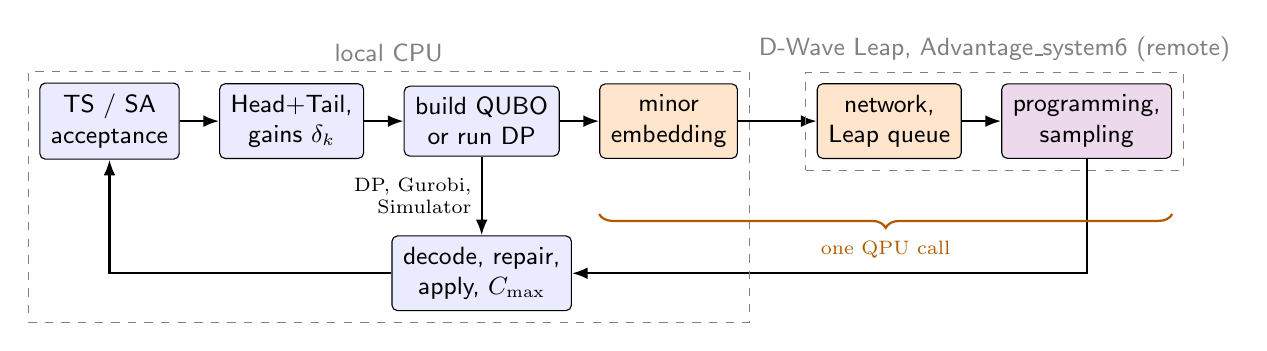
\begin{tikzpicture}[font=\sffamily\small,
  box/.style={draw,rounded corners=2pt,align=center,minimum height=8mm,inner sep=4pt},
  arr/.style={-{Latex[length=2mm]},thick}]
\node[box,fill=blue!8] (meta) {TS / SA\\ acceptance};
\node[box,fill=blue!8,right=5mm of meta] (eval) {Head+Tail,\\ gains $\delta_k$};
\node[box,fill=blue!8,right=5mm of eval] (qubo) {build QUBO\\ or run DP};
\node[box,fill=orange!20,right=5mm of qubo] (emb) {minor\\ embedding};
\node[box,fill=orange!20,right=10mm of emb] (net) {network,\\ Leap queue};
\node[box,fill=violet!15,right=5mm of net] (qpu) {programming,\\ sampling};
\node[box,fill=blue!8,below=10mm of qubo] (dec) {decode, repair,\\ apply, $C_{\max}$};
\draw[arr] (meta)--(eval); \draw[arr] (eval)--(qubo); \draw[arr] (qubo)--(emb);
\draw[arr] (emb)--(net); \draw[arr] (net)--(qpu);
\draw[arr] (qpu.south) |- (dec.east);
\draw[arr] (qubo)--node[left,font=\scriptsize,align=right]{DP, Gurobi,\\ Simulator}(dec);
\draw[arr] (dec.west) -| (meta.south);
\node[draw,dashed,gray,fit=(meta)(eval)(qubo)(emb)(dec),inner sep=4pt,label={[gray]above:local CPU}] {};
\node[draw,dashed,gray,fit=(net)(qpu),inner sep=4pt,label={[gray]above:D-Wave Leap{,} Advantage\_system6 (remote)}] {};
\draw[decorate,decoration={brace,amplitude=5pt,mirror},thick,orange!70!black]
  ([yshift=-7mm]emb.south west) -- node[below=6pt,font=\scriptsize,align=center]{one QPU call}([yshift=-7mm]qpu.south east);
\end{tikzpicture}
\end{center}\textbf{Fig.~1.} Data flow in one iteration of the hybrid algorithm. The minor embedding is computed on the local CPU but belongs to the cost of one QPU call; with the dynamic program, Gurobi or the simulator the iteration stays on the local CPU.}
\change{Section 4, new Fig.~2}{\textit{(no counterpart in the original manuscript)}}{\begin{center}
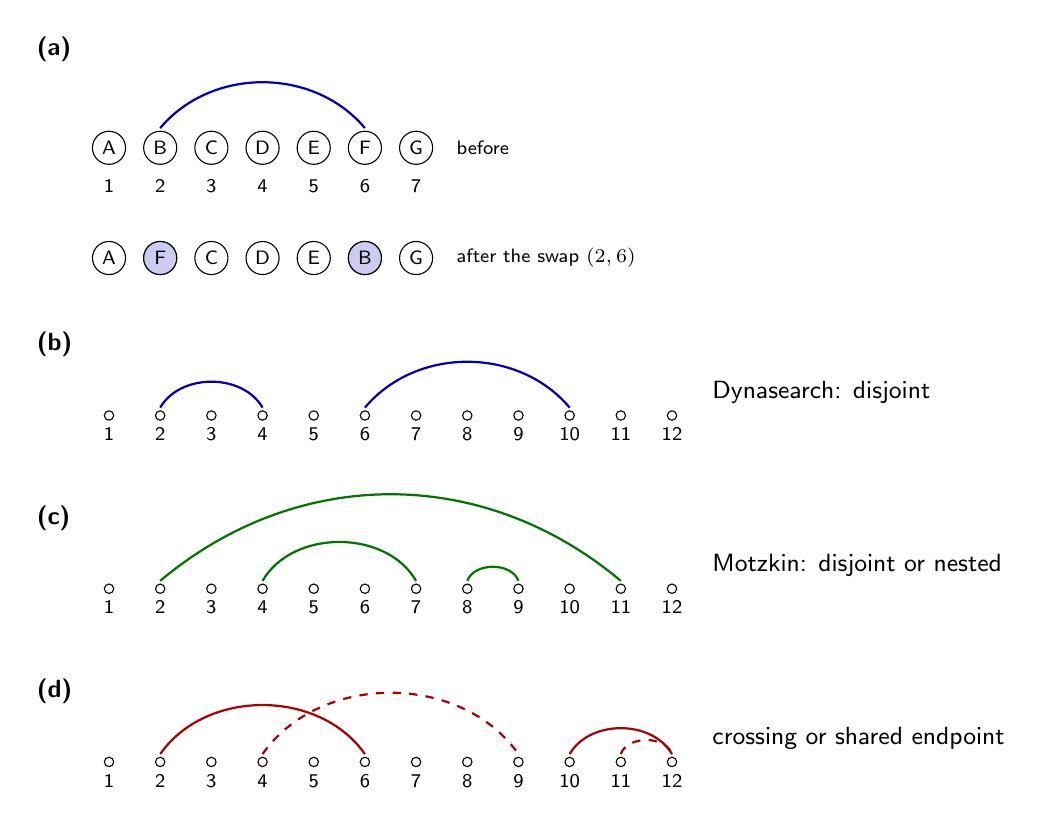
\begin{tikzpicture}[font=\sffamily\scriptsize,x=6.5mm]
% (a) jedna zamiana: przed i po
\node[anchor=west,font=\sffamily\small\bfseries] at (-0.6,1.25) {(a)};
\foreach \i/\j in {1/A,2/B,3/C,4/D,5/E,6/F,7/G} {
  \node[draw,circle,inner sep=1.2pt,minimum size=4.2mm,fill=white] at (\i,0) {\j};
  \node[below=2.5pt] at (\i,-0.2) {\i};
}
\draw[thick,blue!70!black] (2,0.25) to[bend left=50] (6,0.25);
\node[anchor=west] at (7.6,0) {before};
\foreach \i/\j in {1/A,2/F,3/C,4/D,5/E,6/B,7/G} {
  \node[draw,circle,inner sep=1.2pt,minimum size=4.2mm,fill=white] (q\i) at (\i,-1.4) {\j};
}
\node[draw,circle,inner sep=1.2pt,minimum size=4.2mm,fill=blue!70!black!20] at (2,-1.4) {F};
\node[draw,circle,inner sep=1.2pt,minimum size=4.2mm,fill=blue!70!black!20] at (6,-1.4) {B};
\node[anchor=west] at (7.6,-1.4) {after the swap $(2,6)$};
% (b)-(d)
\foreach \y/\lab/\nm in {-3.4/Dynasearch: disjoint/(b),-5.6/Motzkin: disjoint or nested/(c),-7.8/crossing or shared endpoint/(d)} {
  \node[anchor=west,font=\sffamily\small\bfseries] at (-0.6,\y+0.9) {\nm};
  \node[anchor=west,font=\sffamily\small] at (12.6,\y+0.3) {\lab};
  \foreach \i in {1,...,12} { \node[draw,circle,inner sep=1.2pt,fill=white] at (\i,\y) {}; \node[below=1pt] at (\i,\y) {\i}; }
}
\draw[thick,blue!70!black] (2,-3.3) to[bend left=60] (4,-3.3);
\draw[thick,blue!70!black] (6,-3.3) to[bend left=50] (10,-3.3);
\draw[thick,green!45!black] (2,-5.5) to[bend left=40] (11,-5.5);
\draw[thick,green!45!black] (4,-5.5) to[bend left=60] (7,-5.5);
\draw[thick,green!45!black] (8,-5.5) to[bend left=70] (9,-5.5);
\draw[thick,red!65!black] (2,-7.7) to[bend left=55] (6,-7.7);
\draw[thick,red!65!black,dashed] (4,-7.7) to[bend left=55] (9,-7.7);
\draw[thick,red!65!black] (10,-7.7) to[bend left=60] (12,-7.7);
\draw[thick,red!65!black,dashed] (11,-7.7) to[bend left=70] (12,-7.7);
\end{tikzpicture}
\end{center}\textbf{Fig.~2.} Swaps as arcs over job positions. (a)~The swap $(i,j)$ exchanges the jobs at positions $i$ and $j$ and leaves the jobs between them in place; (b)~Dynasearch allows only disjoint arcs, (c)~Motzkin also nested arcs, and (d)~crossing arcs and arcs with a shared endpoint are not allowed.}

\begin{rc}{R1.2 --- Notation $t_{ms}$}
The notation like ``$t_{ms}$'' should be clearly defined in the main text when it is first introduced rather than being inferred from the table captions.
\end{rc}
\answer{We agree. The time budget is now denoted $t_{\max}$ throughout the paper. It is defined in Section~3, where the metaheuristics are introduced, and the same symbol is used in the tables, the figures and the text. The symbol $t_{\mathrm{ms}}$ no longer appears.}
\change{Section 3, opening paragraph}{The algorithm runs within a time budget $t_{\max}$ (in milliseconds) and returns the best-found solution along with the history of improvements in $C_{\max}$ and timestamps of each enhancement.}{Of the methods reviewed in Section~1, we use two local-search metaheuristics that are common for the PFSP, tabu search and simulated annealing. Both start from the identity permutation $\pi=(1,2,\dots,n)$, stop when the wall-clock time budget $t_{\max}$, given in milliseconds, is used up, and return the best permutation found. The budget is checked before every iteration, so an iteration that has already started is completed even if the budget expires in the meantime. The same symbol $t_{\max}$ is used in all tables and figures. In every iteration both methods call the same neighborhood procedure, shown in Algorithm~1, which returns the selected move.}
\change{captions of Tables 2--7}{Average RPD~[\%] from the optimum, $t_{\mathrm{ms}}=100$~ms \textit{(and the five other budgets)}}{Mean RPD~[\%] from the lower bound, $t_{\max}=100$~ms \textit{(and the five other budgets)}}

\begin{rc}{R1.3 --- Qubit count and instance size}
Sentence ``The available qubit count on the QPU additionally bounds the maximum tractable instance size.'' should be more precise.
\end{rc}
\answer{We agree that the sentence was imprecise. The limit comes from minor embedding rather than from the number of qubits alone: every binary variable of a QUBO model occupies a chain of physical qubits, and dense models need long chains. We replaced the sentence with the sizes of the models. For $n=20$ the Adjacent and Fibonacci models have 19 variables, and the Dynasearch and Motzkin models up to 190 variables with up to 13\,110 and 8\,265 quadratic coefficients (Table~1).}
Table 1 is shown under R2~2.3.
\change{Section 7, paragraph Limitations}{The available qubit count on the QPU additionally bounds the maximum tractable instance size.}{\textbf{Limitations.} The experiments were conducted only on instances with $n=20$. The size of the instances is limited by minor embedding rather than by the number of qubits alone. For $n=20$ the Adjacent and Fibonacci models have 19 variables, and the Dynasearch and Motzkin models up to 190 variables with up to 13\,110 and 8\,265 quadratic coefficients (Table~1). A dense model has to be embedded as a clique minor, in which every variable occupies a chain of physical qubits, and the chains grow with the number of variables~[23]. In our runs the embedded Dynasearch and Motzkin models occupied up to 1991 and 1870 physical qubits, with chains of up to 30 and 22 qubits. Already for $n=50$ the unfiltered Dynasearch model would have 1\,225 variables and 519\,400 quadratic coefficients. In a test on the local CPU, the Dynasearch and Motzkin models for $n=50$ could not be embedded into the Advantage processor, which does not have enough qubits for the chains that these dense models need. A precomputed clique embedding, reused in every call, would remove most of the embedding time for the dense models. The SA parameters were set in advance and not tuned, and the results above show that they let SA stagnate. Larger instances need a decomposition of the models, which a separate study addresses~[28].}

\begin{rc}{R1.4 --- Embedding}
What kind of embedding did you use? If QUBO is dense, you can use precomputed clique embedding that is cached, that could reduce embedding time
\end{rc}
\answer{In the experiments of the submitted manuscript we did not use a precomputed or cached embedding. Each QUBO model was sent to the QPU through the \texttt{EmbeddingComposite} of the D-Wave Ocean SDK, which computes a new minor embedding with the heuristic of Cai, Macready and Roy~[23] (the \texttt{minorminer} package) on the local CPU at every QPU call. The chain strength was set by the default rule of the composite (uniform torque compensation), and the time of the embedding was included in the measured wall-clock time of the search. For the sparse Adjacent and Fibonacci models this cost little: a run with the 100~ms budget, which allows a single QPU call, took about 2~s in the median. For the dense Dynasearch and Motzkin models with up to 190 variables the same run took 15~s and 12~s in the median and up to 139~s, so these variants performed about one QPU call per run even at the largest budgets. We agree that this was a weakness of the experimental setup and thank the reviewer for the suggestion.}
In the repeated experiments we kept this setup, so that the results remain comparable with the submitted version, and we measured the time of the embedding separately. For the dense Dynasearch and Motzkin models finding the embedding took 8.4 and 5.4~s in the median, most of a QPU call of 11.0 and 8.2~s, while for the Adjacent and Fibonacci models it took 0.2 and 0.01~s. A precomputed clique embedding, as the reviewer suggests, would remove most of this time for the dense models, and the Limitations paragraph now names it (shown under R1.3).
\change{Section 7, new paragraph QPU}{\textit{(no counterpart in the original manuscript)}}{\textbf{QPU.} In every variant except SA with the Fibonacci neighborhood, where the DP selection itself stagnates, the real QPU, Advantage\_system6, gives the worst schedules at $t_{\max}=10\,000$~ms. The processor takes little of this time. The median QPU access time of one call, which covers programming the processor and 1000 reads, is 0.11 to 0.16~s, while the whole call takes about 2~s for the Adjacent and Fibonacci models and 8 to 11~s for the Dynasearch and Motzkin models. Most of the remaining time goes to finding the minor embedding on the local CPU, 5 to 8~s in the median for the dense models, and to the network and the queue of the Leap service, 1.5 to 2.3~s. Within the budget TS and SA therefore perform 5 or 6 calls with the Adjacent and Fibonacci models and a single call with the Dynasearch and Motzkin models, against thousands of iterations with the DP selection. Figure~4 shows this for TS on one instance: with the DP selection the curves fall within the first second, while the QPU variants of Dynasearch and Motzkin change the schedule once, at the end of the run. The samples of the dense models are also less accurate. For the Adjacent and Fibonacci models the lowest-energy sample was an optimum of the model in more than 99\% of the calls, but for the Dynasearch and Motzkin models only in about a quarter of the calls, and in 62\% and 36\% of the calls it violated the constraints, so the greedy repair had to remove moves.}

\begin{rc}{R1.5 --- Service time and QPU access time}
if possible please additionally provide also service time and QPU access time, that could help reader to understand how much time is used for networking, DWave system queues etc. If the machine was locally installed, the results could be much different as more annealer calls would fit within time limit.
\end{rc}
\answer{We agree, and in the repeated experiments we recorded the components of every QPU call, which Section~7 now reports. The QPU access time, which covers programming the processor and 1000 reads, is 0.11 to 0.16~s in the median. The whole call takes about 2~s for the Adjacent and Fibonacci models and 8 to 11~s for the Dynasearch and Motzkin models. The difference is spent on finding the minor embedding on the local CPU and in the network and queue of the Leap service, 1.5 to 2.3~s. The reviewer is right that a locally installed machine would fit many more calls into the budget: the QPU access time alone would allow several calls per second.}
The new paragraph of Section~7 on the QPU is shown under R1.4.

\begin{rc}{R1.6 --- Number of annealer calls}
I am not sure if using time limit gives enough information, maybe you can add also number of annealer calls (move selections?) and use it for comparison with the number of move selection performed by pure classical versions.
\end{rc}
\answer{We agree. Section~7 now gives the number of QPU calls per run and compares it with the number of iterations of the classical variants. Within $t_{\max}=10\,000$~ms TS and SA performed 5 or 6 QPU calls with the Adjacent and Fibonacci models and a single call with the Dynasearch and Motzkin models (median over the runs). With the DP selection TS performed about 95\,000 iterations with the Adjacent neighborhood, 29\,000 with the Fibonacci neighborhood and 5\,000 to 7\,000 with the Dynasearch and Motzkin neighborhoods. With a single call, the QPU variants of Dynasearch and Motzkin apply one move set to the starting permutation, which is why their results hardly change with the budget.}
The new paragraph of Section~7 on the QPU is shown under R1.4.

% =====================================================================
\newpage

\newpage

\begin{center}
{\bf Answers to the Reviewer \#2 remarks\\[2mm]
``Quantum and Classical Annealing for Very Large-Scale Neighborhood Search in the Permutation Flow Shop Problem''}\\
BPASTS-05673-2026-02\\[5mm]
\end{center}

In the quoted text of the manuscript, reference numbers follow the original manuscript (\textit{Before}) and the revised manuscript (\textit{After}).

\begin{lead}
The article introduces a QUBO formulation framework for heuristic neighborhood structures for the Permutation Flow Shop Scheduling Problem (PFSP) within a hybrid classical--quantum optimization framework. The proposed approach is evaluated using a D-Wave quantum annealer.

The topic is interesting and potentially relevant to the application of quantum optimization methods to scheduling problems. However, the manuscript requires substantial improvement in terms of structure, clarity, and methodological rigor. Several sections are difficult to follow, and important aspects of the proposed methodology are insufficiently explained or justified.
\end{lead}

\begin{rc}{R2.G1 --- QUBO formulation versus quantum computing}
In particular, the manuscript does not consistently distinguish between QUBO formulations and quantum computing as an optimization paradigm. A QUBO formulation can be solved using either classical or quantum algorithms; therefore, the use of a QUBO formulation does not, by itself, imply the use of quantum computing. This distinction should be made explicit throughout the manuscript, and the terminology should be revised accordingly.
\end{rc}
\answer{We agree. The revised manuscript keeps three notions apart throughout: the neighborhood (the set of admissible move sets), the selection model (a dynamic program or a QUBO model) and the solver (the dynamic program on a CPU or, for the QUBO model, Gurobi, a classical sampler or sampling on a QPU). The names ``Quantum Adjacent'' and similar were removed, the variants are named by the neighborhood and the solver, and the word ``quantum'' is used only where the QPU is involved. The title now states that the move selection, not the neighborhood, is either classical or performed by quantum annealing, and it names tabu search instead of iterated local search (see the response to the remark on Iterated Local Search). The abstract says explicitly that the same QUBO model can be solved by a classical algorithm or sampled on a quantum annealer.}
\change{title}{Classical and Quantum Neighborhoods Evaluation in Iterated Local Search and Simulated Annealing for the Permutation Flow Shop Problem}{Quantum and Classical Annealing for Very Large-Scale Neighborhood Search in the Permutation Flow Shop Problem}
\change{running title}{Classical and Quantum Neighborhoods Evaluation in PFSP}{Quantum and Classical Annealing for Neighborhood Search in PFSP}
\change{abstract}{This paper presents a comparison of classical neighborhood structures, analyzed from an implementation perspective in metaheuristics, with their hybrid classical--quantum counterparts. The study is conducted for the Permutation Flow Shop Scheduling Problem (PFSP), where classical neighborhood structures are executed entirely on a classical computing architecture (CPU), while their quantum counterparts are implemented in a hybrid manner, combining classical computations with the use of a real Quantum Processing Unit (QPU). The optimization objective is to minimize the makespan, i.e., the total completion time of all jobs on all machines, denoted as $C_{\max}$. Four classical neighborhood structures are considered: \emph{Adjacent}, \emph{Fibonacci}, \emph{Dynasearch}, and \emph{Motzkin}, along with their quantum counterparts formulated as Quadratic Unconstrained Binary Optimization (QUBO) models, namely: \emph{Quantum Adjacent}, \emph{Quantum Fibonacci}, \emph{Quantum Dynasearch}, and \emph{Quantum Motzkin}. The considered structures differ in terms of move generation mechanisms within the permutation space and computational complexity. The paper provides a detailed characterization of each neighborhood structure and its corresponding QUBO formulation. The proposed models are implemented in \texttt{Python} using the \texttt{dimod} library and experimentally validated on standard Taillard benchmark instances, using both classical CPU-based computations and a real QPU, enabling the assessment of the quality of the obtained solutions.}{Compound neighborhoods for the permutation flow shop problem apply several compatible moves in one step, and choosing these moves is itself an optimization problem. We study this move selection step for four neighborhoods, Adjacent, Fibonacci, Dynasearch and Motzkin, used inside tabu search and simulated annealing to minimize the makespan. For each neighborhood the selection can be solved exactly by dynamic programming, and we also write it as a quadratic unconstrained binary optimization (QUBO) model. We give penalty weights that make every minimizer of these models feasible, the structure of their coefficient matrices and the cost of building them, and we keep the model separate from the solver: the same QUBO model can be solved by a classical algorithm or sampled on a quantum annealer. In the experiments the move selection is performed in four ways on Taillard instances with 20 jobs under equal wall-clock budgets: by dynamic programming, and by solving the QUBO model exactly with the Gurobi solver, approximately with a classical simulated annealing sampler, or by sampling on a real quantum processing unit (QPU), the D-Wave Advantage\_system6 quantum annealer, accessed through the Leap cloud service. Solving the models on a classical computer gives worse schedules than dynamic programming in most variants, because one call of a QUBO solver takes up to thousands of times longer, so the search performs fewer iterations within the same budget. On the QPU the schedules are worse still, because most of a call is spent outside the processor, on finding the minor embedding and in the network and queue of the cloud service, so the dense models allow about one call within ten seconds.}
\change{keywords}{Flow shop scheduling; QUBO; Quantum computing; D-Wave; Neighborhood; Metaheuristics; Motzkin numbers; Fibonacci numbers}{Permutation flow shop; Neighborhood search; Dynamic programming; QUBO; Quantum annealing; Very large-scale neighborhood search; D-Wave}
\change{Tables 2--7, now Tables 2 and 3}{Six tables, one per time budget, with columns \textit{Type} (Classic / Quantum), \textit{Method} (ILS / SA) and \textit{Neighborhood} (adj, \dots, q-adj, \dots).}{Two tables, one for TS and one for SA, with rows \textit{Solver} (Classical DP / Gurobi / Simulator / QPU) and \textit{Neigh.} (adj, fib, dyn, mot) and one group of columns for each time budget; the lowest value in each column is in bold.}
The new paragraph of Section~7 on the QUBO models solved classically is shown under R2~5.
\medskip

\begin{rc}{R2.G2 --- Balance of the reference list}
Furthermore, the reference list appears unbalanced. The manuscript would benefit from a broader discussion of established research in operations research, particularly concerning the PFSP, exact and heuristic scheduling methods, QUBO formulations, and quantum annealing. The relatively frequent citation of works by R.~Wojewódzki and W.~Bożejko should be complemented by a more comprehensive selection of relevant literature.
\end{rc}
\answer{We agree. The Introduction now reviews foundational work on the PFSP, exact methods (branch and bound and mixed-integer programming), constructive heuristics and metaheuristics, compound and very large-scale neighborhoods, QUBO models and quantum annealing, including applications to scheduling. The Introduction alone now cites 28 works instead of 5, and 23 of the works cited there are by other authors. We removed two self-citations, one unrelated to the subject of the paper and one on parallel neighborhood search that the paper does not need, and replaced an incorrect reference for Dynasearch. The remaining citations of works by these authors define the Fibonacci and Motzkin neighborhoods used in the paper, report earlier work on quantum annealing for scheduling, or describe the preprint discussed in the next point.}
\change{Section 2, former second paragraph}{Properties of permutations and the relationships between them can be analyzed using positive definite functions on permutation groups. This provides theoretical foundations for studying dependencies between job sequences~[6].}{\textit{(removed, together with the reference)}}
\par\smallskip\noindent\textbf{Change in the manuscript (Introduction, paragraphs 1--7).} The new text of the Introduction, with its references, is shown under points R2.1a--R2.1e and R2.G3 below.\par
\change{reference for Dynasearch}{D.~Campos-Rodr\'iguez et al.\ (old [43], an unrelated paper on scatter search for linear ordering)}{R.~K.~Congram, C.~N.~Potts and S.~L.~van de Velde, An iterated dynasearch algorithm for the single-machine total weighted tardiness scheduling problem, INFORMS J.\ Comput.\ 14(1), 2002 [21]}

\begin{rc}{R2.G3 --- Relation to SSRN 7411334}
There may also be some overlap with the following recent work:

Wojewódzki, R., \& Bożejko, W. \emph{Scalable Quantum Neighborhood Search for the Permutation Flow Shop Problem via Windowed QUBO Decomposition}. Available at SSRN, No.~7411334.

The authors should clarify the relationship between the two contributions and explicitly identify the methodological and experimental differences. In particular, the novelty of the proposed neighborhood formulations, their QUBO encodings, and the experimental evaluation should be established relative to this and other closely related studies.
\end{rc}
\answer{The preprint builds on the QUBO models of the present manuscript and cites the manuscript as their source. The two works differ in aim and scope. The present manuscript formulates the move selection of the four neighborhoods as whole QUBO models, so that the QPU solves exactly the problem that dynamic programming solves, and compares the two selections inside two metaheuristics on instances with 20 jobs, where the whole models fit the processor. The preprint addresses scalability. It drops the removal of non-improving candidates, reduces the candidate set with block properties of the critical path, splits the Dynasearch and Motzkin models into overlapping windows of at most 19 positions that are solved one after another, uses a different restart strategy and reports experiments with up to 500 jobs. It also runs the whole models for 20 jobs, but in a separate campaign with other settings and only as a reference point for the decomposed models. The derivations of the models, their structure and penalty weights, and the comparison of the exact and the QPU selection under equal budgets appear only in the present manuscript. A paragraph at the end of the Introduction now states this relation and cites the preprint.}
\change{Introduction, new paragraph 7}{\textit{(no counterpart in the original manuscript)}}{The preprint~[28] builds on the QUBO models of the present paper. It modifies them and splits the Dynasearch and Motzkin models into overlapping windows that are solved one after another, which lets it run instances with up to 500 jobs. The present paper keeps every model whole, so that the QPU solves exactly the selection problem that dynamic programming solves, and studies the cost of this delegation on instances with 20 jobs.}

\begin{lead}
The following comments provide more detailed suggestions for improving the manuscript.
\end{lead}

\subsection*{1. Introduction}

\begin{lead}
The structure and content of the Introduction require substantial improvement. I recommend reorganizing this section as follows.
\end{lead}

\begin{rc}{R2.1a --- Foundational references on flow shop scheduling}
In the first paragraph, please include additional well-established references on the Flow Shop Scheduling Problem, particularly foundational and widely cited studies.
\end{rc}
\answer{We agree. The first paragraph now cites foundational work on the flow shop problem: Johnson's two-machine algorithm, the NP-hardness proof of Garey, Johnson and Sethi, the three-field notation of Graham et al., Taillard's benchmark and the review of Ruiz and Maroto.}
\change{Introduction, paragraph 1}{The Permutation Flow Shop Scheduling Problem (PFSP) is a classical combinatorial optimization problem, in which $n$ jobs must be processed on $m$ machines in the same sequence on each machine. The objective is to minimize the makespan $C_{\max}$, i.e., the completion time of the last job on the last machine. It is well-known that the problem is NP-hard for $m \ge 3$, rendering exact methods computationally inefficient for large instances and motivating the use of metaheuristic approaches~[1].}{In the permutation flow shop scheduling problem (PFSP), $n$ jobs are processed on $m$ machines, every job visits the machines in the same order, and every machine processes the jobs in the same sequence. The goal is a sequence that minimizes the makespan $C_{\max}$, the completion time of the last job on the last machine. Johnson~[1] gave a polynomial algorithm for two machines, and Garey, Johnson and Sethi~[2] proved the problem NP-hard for $m\ge 3$. In the three-field notation of Graham et al.~[3] it is written $F_m|prmu|C_{\max}$. It is one of the most studied scheduling problems, reviewed by Ruiz and Maroto~[4], and the instances of Taillard~[5] are the standard benchmark for its solution methods.}

\begin{rc}{R2.1b --- Overview of classical PFSP methods}
Before introducing quantum computing, the manuscript should provide a concise overview of established approaches to solving the PFSP. This discussion should cover both exact methods, such as branch-and-bound algorithms and mathematical programming approaches, and heuristic or metaheuristic methods.
\end{rc}
\answer{We agree. A new second paragraph of the Introduction reviews exact methods, namely branch-and-bound algorithms and mixed-integer programming models, and heuristic methods, from the NEH heuristic to simulated annealing, tabu search and iterated greedy, before quantum computing is introduced.}
\change{Introduction, new paragraph 2}{\textit{(no counterpart in the original manuscript)}}{Exact methods for the PFSP are mainly branch-and-bound algorithms~[6] and mixed-integer programming models~[7]. They prove optimality for small and medium instances, but their running time grows quickly with the number of jobs and machines, so large instances are solved heuristically. The constructive heuristic NEH~[8] is still a common starting point. Improvement methods are mostly metaheuristics based on local search, such as simulated annealing~[9], tabu search~[10, 11, 12] and iterated greedy~[13].}

\begin{rc}{R2.1c --- Order of paragraphs}
The current second paragraph should be moved to a position following the discussion of classical PFSP solution methods. This would establish the scheduling context before introducing quantum optimization.
\end{rc}
\answer{We agree. The former second paragraph, on neighborhoods, now follows the review of classical methods, and quantum annealing is introduced only after it. Both paragraphs were also rewritten: the paragraph on neighborhoods now cites the original work on Dynasearch and on very large-scale neighborhood search, and the paragraph on quantum annealing covers the Ising and QUBO models, minor embedding and applications of quantum annealing to scheduling.}
\change{Introduction, former paragraph 2, now paragraph 3}{In the context of metaheuristic algorithms, a \emph{neighborhood} of a solution $\pi$ is defined as the set of solutions reachable from $\pi$ by a single permissible modification~[2]. The structure and size of the neighborhood determine both the quality of the solutions obtained and the computational cost of a single iteration. Simple neighborhoods, such as adjacent swaps, allow for a high number of iterations per unit of time, but explore the solution space in a limited scope. More complex neighborhoods, such as Dynasearch or Motzkin, enable larger modifications of the permutation but require higher computational effort per step~[3, 4].}{A local-search metaheuristic moves from a solution $\pi$ to a solution in its neighborhood, the set of solutions reachable from $\pi$ by one admissible modification. The neighborhood decides how much one step can improve the solution and how much the step costs. Simple neighborhoods, such as the swap of two adjacent jobs, are cheap to evaluate but change the sequence only locally. Compound neighborhoods apply several compatible moves in one step and may contain exponentially many solutions. Dynasearch~[14] searches such a neighborhood of independent swaps exactly by dynamic programming, and it belongs to the wider family of very large-scale neighborhood search methods~[15]. The Fibonacci~[16] and Motzkin~[17, 18] neighborhoods are compound neighborhoods of the same kind, and their numbers of move sets are given by the Fibonacci and Motzkin numbers.}
\change{Introduction, first part of former paragraph 3, now paragraph 4}{Quantum computing provides an alternative paradigm for solving combinatorial optimization problems. Quantum annealers, such as the D-Wave system, solve Quadratic Unconstrained Binary Optimization (QUBO) problems, which can encode a wide range of optimization and constraint satisfaction tasks~[5].}{A quantum annealer samples low-energy states of an Ising model~[19, 20]. The Ising model is equivalent to quadratic unconstrained binary optimization (QUBO), in which many combinatorial problems can be written~[21, 22]. A QUBO model can also be solved by classical algorithms, so writing a problem as a QUBO does not by itself mean using a quantum computer. To run on the processor, the graph of the model must be minor-embedded into the sparse graph of the hardware, and one binary variable may then occupy a chain of several physical qubits~[23]. Applications to scheduling mostly encode the whole schedule as one QUBO, for example for the job shop~[24], and such encodings have been solved on the hardware only for small instances~[25]. Kurowski et al.~[26] combined an annealer with a classical heuristic for the job shop, and Bożejko et al.~[27] applied distributed quantum annealing on D-Wave to the single-machine total weighted tardiness problem.}

\begin{rc}{R2.1d --- Claim about the quantum annealer}
The following statement is too strong:

``The quantum annealer then enables the selection of the best permissible combination of swaps in a single optimization step, potentially considering a significantly larger number of combinations than classical greedy or dynamic approaches.''

Quantum annealers are subject to hardware and embedding constraints, limited connectivity, noise, finite sampling budgets, and other limitations associated with current quantum technologies. Consequently, the statement that a quantum annealer selects the best permissible combination of swaps should be qualified. Please distinguish between finding an optimal solution to the mathematical QUBO model and obtaining a high-quality candidate solution using a real quantum device. Any claimed advantage over classical methods should be supported by experimental evidence.
\end{rc}
\answer{We agree, and we removed the statement. It was too strong, and its comparison with dynamic programming was wrong. For the four neighborhoods, dynamic programming solves the same selection problem exactly in polynomial time, so the annealer cannot find a better combination of moves. At best it finds the same one, and noise, embedding and a finite number of samples may lead it to a worse one. The revised Introduction distinguishes the optimum of the QUBO model from a sample returned by the device. It also notes that both selections minimize the sum of individually evaluated gains, which only approximates the change of the makespan, and it states that the paper measures the cost of delegating the selection to the QPU rather than an advantage over classical methods.}
\change{Introduction, second part of former paragraph 3, now paragraph 5}{The key idea of this work is to transform the neighborhood move selection — i.e., the decision of which swaps to perform — into a QUBO problem. The quantum annealer then enables the selection of the best permissible combination of swaps in a single optimization step, potentially considering a significantly larger number of combinations than classical greedy or dynamic approaches.}{In this paper the annealer works inside a metaheuristic instead of replacing it. The metaheuristic runs on a classical computer, and in every iteration only the move selection step, the choice of a set of mutually compatible moves, is written as a QUBO model and sent to a real quantum processing unit (QPU), the D-Wave Advantage\_system6 annealer accessed through the Leap cloud service. We call such an algorithm hybrid. Three terms are kept apart throughout the paper. The \emph{neighborhood} is the set of admissible move sets. The \emph{selection model} is the optimization problem that picks one of these sets, written either as a dynamic program or as a QUBO model. The \emph{solver} is the method that solves this model: the dynamic program on the CPU or, for the QUBO model, the exact solver Gurobi, a classical simulated annealing sampler or sampling on the QPU. For all four neighborhoods studied here, dynamic programming solves the selection problem exactly in polynomial time. A quantum annealer therefore cannot return a better selection than the classical procedure. At best it returns the same set, and noise, minor embedding and a finite number of samples may lead it to a worse one. For the compound neighborhoods both procedures also minimize the sum of individually evaluated move gains, which only approximates the change of the makespan. Our question is therefore not whether the annealer selects better moves, but how much solution quality and time it costs to delegate an exactly solvable selection step to a remote QPU, and where this cost comes from.}

\begin{rc}{R2.1e --- ``Classical'' and ``hybrid neighborhoods''}
The following statement is unclear:

``QUBO-based formulations and provides an experimental comparison of classical and hybrid neighborhoods using a real QPU.''

Please clarify what is meant by ``classical neighborhoods'' and ``hybrid neighborhoods.'' In particular, does the latter term refer to classical neighborhood structures encoded as QUBO models and submitted to a quantum processing unit, or does it refer to a hybrid optimization algorithm in which classical and quantum computations perform different tasks? The terminology should be defined explicitly and used consistently throughout the manuscript.
\end{rc}
\answer{We agree. The Introduction now defines the terms (paragraph 5, shown under R2.1d). A neighborhood is a set of admissible move sets, the selection model is a dynamic program or a QUBO model, and a hybrid algorithm is a metaheuristic running on a CPU that sends the selection model to the QPU in every iteration. The expression ``hybrid neighborhood'' was removed, and the variants are named by the neighborhood and the solver throughout.}
\change{Introduction, former paragraph 4, now paragraph 6}{This paper emphasizes the transformation of classical neighborhood structures into their corresponding QUBO-based formulations and provides an experimental comparison of classical and hybrid neighborhoods using a real QPU. The study aims to assess the potential of quantum acceleration in solving scheduling problems. While~[4] and~[3] introduced the classical Motzkin and Fibonacci neighborhoods, the present work makes three distinct contributions: (i)~it formulates all four classical neighborhoods as QUBO problems executable on a quantum annealer, (ii)~it provides the first empirical comparison of classical and quantum variants under identical wall-clock time budgets on real QPU hardware, and (iii)~it identifies and quantifies the sources of the performance gap between classical and quantum approaches.}{The contribution of the paper is as follows. We write the move selection of the Adjacent, Fibonacci, Dynasearch and Motzkin neighborhoods as QUBO models, give penalty weights that make every minimizer feasible, and state the number of variables, the number of nonzero quadratic coefficients and the cost of building each model. We give the dynamic programs that solve the same selection problems exactly, with their complexity. We then compare four ways of selecting the move inside tabu search and simulated annealing under equal wall-clock budgets on Taillard instances with 20 jobs: the dynamic program, and the QUBO model solved exactly by Gurobi, approximately by a classical simulated annealing sampler, and on the real D-Wave QPU. Solving the same QUBO model on a classical computer separates the cost of the model from the cost of the quantum processor, and we discuss which parts of a QPU call slow the hybrid variants down. The Fibonacci and Motzkin neighborhoods and their classical selection were introduced in~[16, 17, 18]; the QUBO models and their comparison with the dynamic programs are new in this paper.}
The new layout of Tables 2--7 is shown under R2.G1, and the new paragraph of Section~7 on the QUBO models solved classically under R2~5.

\subsection*{2. Problem Definition: Permutation Flow Shop Scheduling Problem}

\begin{rc}{R2.2 --- Structure of Section 2}
The structure of this section is difficult to follow. After introducing the PFSP in a somewhat unclear manner, the authors discuss heuristic solution methods and then move directly to neighborhood structures. The discussion would benefit from a more systematic organization.

In particular, the section should first define the scheduling problem, its assumptions, and its objective function. It should then briefly review relevant exact and heuristic solution methods before introducing the neighborhood structures used in the proposed approach.
\end{rc}
\answer{We agree. Section~2 now contains only the definition of the problem: its assumptions, the notation, the completion-time recurrence and the objective. Section~3 opens with a link to the exact and heuristic methods reviewed in the Introduction and then describes the two metaheuristics, and the neighborhood structures follow in Section~4.}
\change{structure of Sections 2--4}{Section~2 (Problem Definition) contained the definition of the PFSP, a remark on positive definite functions on permutation groups, the descriptions of iterated local search and simulated annealing, and the neighborhood structures.}{Section~2 (Problem Definition) contains only the problem: assumptions, notation, the recurrence and the objective. Section~3 (Search Methods) describes tabu search and simulated annealing and gives Algorithm~1. Section~4 (Neighborhood Structures) describes the four neighborhoods.}
The new opening paragraph of Section~3 is shown under R1.2, and the new text of Section~2 under R2.2a--R2.2c.

\begin{lead}
My specific comments are as follows.
\end{lead}

\begin{rc}{R2.2a --- Three-field notation}
Please introduce the PFSP more intuitively and consider using the standard three-field scheduling notation:
\[ F_m \,|\, prmu \,|\, \Cmax . \]
The notation should be explained, including the meaning of the permutation constraint.
\end{rc}
\answer{We agree. The problem is now first described in words and then written as $F_m|prmu|\Cmax$, with each field explained. The explanation includes the permutation constraint: all machines process the jobs in the same order, so a schedule is a single permutation.}
\change{Section 2, end of the first paragraph}{\textit{(no counterpart in the original manuscript)}}{In the three-field notation of Graham et al.~[3] the problem is $F_m|prmu|C_{\max}$: the first field denotes a flow shop with $m$ machines, the second the permutation constraint, and the third the makespan objective.}

\begin{rc}{R2.2b --- Optimization objective}
Please state the optimization objective explicitly, namely the minimization of the makespan $\Cmax$.
\end{rc}
\answer{We agree. The objective, the minimization of $\Cmax(\pi)=C_{m,n}$ over all permutations, is now stated explicitly as an equation.}
\change{Section 2, objective}{The value of the objective function equals $C_{\max} = C_{m,n}$, i.e., the completion time of the last job on the last machine. Hence, the PFSP reduces to finding a permutation $\pi$ that minimizes $C_{\max}$.}{The makespan of $\pi$ is $C_{\max}(\pi)=C_{m,n}$, the completion time of the last job on the last machine, and the problem is to find
\begin{equation}
\pi^* = \arg\min_{\pi\in\Pi_n} C_{\max}(\pi).
\end{equation}
The recurrence computes $C_{\max}(\pi)$ in $O(mn)$ time.}

\begin{rc}{R2.2c --- Notation and boundary conditions of the recurrence}
The mathematical notation and accompanying explanations should be improved. In particular, define the quantities explicitly, for example:
\begin{itemize}[label=-]
\item $\pi(j)$: the job occupying position $(j)$ in the common processing sequence.
\end{itemize}
The completion-time recurrence should be presented with clearly defined boundary conditions. For example,
\begin{align*}
C_{1,1} &= p_{1,\pi(1)},\\
C_{1,j} &= C_{1,j-1}+p_{1,\pi(j)}, & j &= 2,\ldots,n,\\
C_{k,1} &= C_{k-1,1}+p_{k,\pi(1)}, & k &= 2,\ldots,m,\\
&\;\;\ldots
\end{align*}
These definitions would eliminate the ambiguity arising from the current use of boundary cases in the recurrence relations.
\end{rc}
\answer{We agree. $\pi(j)$ and $p_{k,\pi(j)}$ are defined before they are used, and the recurrence is given with separate boundary conditions, as the reviewer suggested. This also removes an inconsistency of the previous version, in which the general formula was stated for $k=1$ and $j=1$ as well.}
\change{Section 2, definition and recurrence}{Given a matrix of processing times $P = [p_{k,j}]_{m \times n}$, where $k=1,\dots,m$ denotes a machine and $j=1,\dots,n$ denotes a job, while a permutation $\pi$ determines the jobs performed in the same order on all machines.

Let $C_{k,j}$ denote the completion time of job $j$ executed in the order $\pi$ on machine $k$. The following relationship therefore holds:

\begin{equation}
    C_{1,j} = C_{1,j-1} + p_{1,\pi(j)},\quad
    C_{k,1} = C_{k-1,1} + p_{k,\pi(1)},
\end{equation}

\begin{equation}
\begin{aligned}
C_{k,j} &= \max\{C_{k,j-1},\, C_{k-1,j}\} + p_{k,\pi(j)}, \\
        &\text{for } k=1,\dots,m,\; j=1,\dots,n.
\end{aligned}
\end{equation}}{We are given a set of $n$ jobs $J=\{1,\dots,n\}$ and a set of $m$ machines $M=\{1,\dots,m\}$. Every job visits the machines in the order $1,2,\dots,m$, and job $j$ occupies machine $k$ for $p_{k,j}>0$ time units. All jobs are available at time zero, a machine processes at most one job at a time, a job is processed by at most one machine at a time, and an operation cannot be interrupted. In the permutation flow shop all machines process the jobs in the same order. A schedule is therefore described by one permutation $\pi=(\pi(1),\dots,\pi(n))$ of $J$, where $\pi(j)$ is the job at position $j$ of the common sequence, and $\Pi_n$ denotes the set of all $n!$ such permutations. In the three-field notation of Graham et al.~[3] the problem is $F_m|prmu|C_{\max}$: the first field denotes a flow shop with $m$ machines, the second the permutation constraint, and the third the makespan objective.

Let $C_{k,j}$ denote the completion time of the job at position $j$ on machine $k$. The completion times follow from the recurrence
\begin{align}
C_{1,1} &= p_{1,\pi(1)}, \\
C_{1,j} &= C_{1,j-1}+p_{1,\pi(j)}, \quad j=2,\dots,n, \\
C_{k,1} &= C_{k-1,1}+p_{k,\pi(1)}, \quad k=2,\dots,m, \\
C_{k,j} &= \max\{C_{k-1,j},\,C_{k,j-1}\}+p_{k,\pi(j)}, \nonumber\\
&\qquad k=2,\dots,m,\ j=2,\dots,n. 
\end{align}}

\begin{rc}{R2 ILS --- Tabu list in Iterated Local Search}
Standard Iterated Local Search does not inherently include a tabu list. Its defining components are typically local search, perturbation, and an acceptance criterion. A tabu mechanism can be incorporated into an ILS variant, but this should be identified as an additional algorithmic component. Please specify.
\end{rc}
\answer{We agree. Our algorithm moves in every iteration to the best admissible neighbor, uses a tabu list with an aspiration criterion and restarts from a random permutation when the compound move returned by the neighborhood is tabu. It has no separate local-search and perturbation phases, so it is tabu search with restarts rather than iterated local search. We renamed it tabu search (TS) throughout the paper, described all its components (move selection, tabu list, aspiration and restart) and added references to tabu search for the PFSP.}
\change{Section 3, description of the first metaheuristic}{\textbf{Iterated Local Search} (ILS)~[7] combines local search with a tabu list to avoid cyclic revisiting of the same solutions. In each iteration, the algorithm identifies the best neighboring solution and checks whether the corresponding move is on the tabu list~[8]. A move is accepted despite being tabu if it satisfies the \emph{aspiration criterion}, i.e., it leads to a solution better than the current best.

The tabu list stores forbidden moves for $\tau$ consecutive iterations (\emph{tabu tenure}, \texttt{tabu\_tenure}). For the \emph{Adjacent} and \emph{Fibonacci} neighborhoods, the algorithm selects the $\tau + 1$ best moves and chooses the first non-tabu move, ensuring the search can continue even with a full tabu list. For the remaining neighborhoods — \emph{Dynasearch}, \emph{Motzkin}, and their quantum counterparts — any conflict with the tabu list triggers a random restart: a new permutation is generated to replace the current solution, and its identifier is added to the tabu list.

The algorithm runs within a time budget $t_{\max}$ (in milliseconds) and returns the best-found solution along with the history of improvements in $C_{\max}$ and timestamps of each enhancement.}{\textbf{Tabu search.} Tabu search (TS)~[29] moves in every iteration to the best admissible solution returned by the neighborhood procedure, even if it is worse than the current one. A tabu list keeps an identifier of every executed move for $\tau$ iterations (the tabu tenure) and forbids repeating it, which keeps the search from cycling back to recently visited solutions. A tabu move is still accepted if it satisfies the aspiration criterion, that is, if it gives a solution better than the best one found so far. With exact selection, the Adjacent and Fibonacci procedures return their $\tau+1$ best moves, and the search takes the best of them that is not tabu, so a non-tabu move is always available. The Dynasearch and Motzkin procedures and all QPU variants return a single move. If this move is tabu and does not satisfy the aspiration criterion, the search restarts from a random permutation, which is added to the tabu list. The method has no separate perturbation phase, and the restart is its only diversification step. Tabu search is a standard method for the PFSP~[10, 11, 12].}

\begin{rc}{R2 SA (a) --- Interpretation of the temperature}
Please clarify the interpretation of the temperature parameter $T$. In a scheduling metaheuristic, it is an algorithmic control parameter inspired by physical annealing, rather than a physical temperature.
\end{rc}
\answer{We agree. The description now states that $T$ is a control parameter of the algorithm, measured in the units of the makespan, with no relation to a physical temperature. We added this remark also because the paper uses simulated annealing and quantum annealing side by side.}
\change{Section 3, simulated annealing, first part}{\textbf{Simulated Annealing}(SA)~[9] is a local search metaheuristic inspired by the annealing process in metallurgy. In each iteration, the algorithm generates a neighboring solution and accepts it unconditionally if it improves the objective function, or with Boltzmann probability $\exp(-\Delta/T)$ if it worsens it, where $\Delta = C_{\max}^{\text{new}} - C_{\max}^{\text{cur}}$ is the change in the objective function and $T$ is the current temperature. This mechanism allows the search to escape local minima, with the likelihood of accepting worsening moves decreasing as the temperature drops.}{\textbf{Simulated annealing.} Simulated annealing (SA)~[30, 9] accepts worse solutions with a probability that decreases during the search. In our implementation the neighborhood procedure returns its best move, as in TS, and the Metropolis rule decides whether the search moves to it: a move that changes the makespan by $\Delta=C_{\max}^{\text{new}}-C_{\max}^{\text{cur}}$ is always accepted if $\Delta\le 0$ and is accepted with probability $\exp(-\Delta/T)$ otherwise. The temperature $T$ is a control parameter of the algorithm, measured in the units of the makespan. It has no relation to a physical temperature, nor to the physics of the quantum annealer used later in the paper.}

\begin{rc}{R2 SA (b) --- Roles of $T_{final}$ and $f$}
Please explain the roles of $T_{final}$ and the parameter $f$. As these parameters are mathematically dependent, please explain why both are required and how they are selected.
\end{rc}
\answer{The reviewer is right that one of the two parameters was redundant. In all experiments $f=1$, so the lowest temperature was $T_{\text{final}}$, and we removed $f$ from the description. Section~6 now gives the values of the remaining parameters and their effect: the temperature decreases from $T_{\text{init}}=1000$ to $T_{\text{final}}=1$ with $\alpha=0.95$, which takes 135 iterations. These values were set in advance and not tuned, and Section~7 discusses their effect on the results.}
\change{Section 3, simulated annealing, cooling rule}{The temperature is geometrically reduced after each iteration according to $T \leftarrow \max(T \cdot \alpha,\, T_{\min})$, where $\alpha \in (0,1)$ is the cooling rate, and $T_{\min} = T_{\text{final}} \cdot f$ is a lower bound set by the floor parameter $f \ge 1$.}{After every iteration the temperature is lowered geometrically, $T\leftarrow\max(\alpha T,\,T_{\text{final}})$, from the initial value $T_{\text{init}}$, where $\alpha\in(0,1)$ is the cooling rate and $T_{\text{final}}$ the lowest temperature.}
\change{Section 6, parameters}{SA: $T_{\text{init}}=1000$, $T_{\text{final}}=1$, $\alpha=0.95$, reheating factor $r = 1.5$, stagnation threshold $500$~(ms).}{SA used $T_{\text{init}}=1000$, $T_{\text{final}}=1$ and $\alpha=0.95$, so its temperature reaches $T_{\text{final}}$ after 135 iterations, and reheating with $r=1.5$ and $t_{\text{stag}}=500$~ms. The segments of Dynasearch and Motzkin were not limited in length. These values were set in advance and not tuned.}

\begin{rc}{R2 SA (c) --- Reheating after stagnation}
The following description requires clarification:

``If no improvement in the best solution is observed for at least $t_{stag}$ milliseconds, the temperature is multiplied by a factor $r>1$ and restored to at most $T_{init}$. The algorithm runs within the time budget $t_{\max}$ (in milliseconds) and returns the best-found solution upon termination.''

Increasing the temperature after a period of stagnation is a modification of conventional Simulated Annealing, rather than a standard cooling rule. Please explain the motivation for this mechanism in more detail.
\end{rc}
\answer{We agree that reheating is a modification of the standard cooling rule, and Section~3 now explains its motivation. With geometric cooling the temperature reaches $T_{\text{final}}$ after a fixed number of iterations, 135 with our parameters, and from then on SA accepts almost no worse moves. Reheating is meant to let a long run leave a local optimum after this point: if the best solution has not improved for $t_{\text{stag}}$ milliseconds, the temperature is multiplied by a factor $r>1$, but not above $T_{\text{init}}$. In our experiments, with $r=1.5$ and $t_{\text{stag}}=500$~ms, reheating had no visible effect. The RPD of every SA variant with DP selection is the same for all budgets, because the following iterations lower the raised temperature back to $T_{\text{final}}$ within eight steps. Section~7 states this and explains why SA stagnates.}
\change{Section 3, simulated annealing, reheating}{To prevent stagnation, a reheating mechanism is implemented: if no improvement in the best solution is observed for at least $t_{\text{stag}}$ milliseconds, the temperature is multiplied by a factor $r > 1$ and restored to at most $T_{\text{init}}$.}{With this schedule the temperature reaches $T_{\text{final}}$ after $\lceil\ln(T_{\text{final}}/T_{\text{init}})/\ln\alpha\rceil$ iterations, and from then on SA accepts almost no worse moves. Reheating is a modification of the standard cooling rule that is meant to let a long run leave a local optimum after this point: if the best solution has not improved for $t_{\text{stag}}$ milliseconds, the temperature is multiplied by a factor $r>1$, but not above $T_{\text{init}}$, and the stagnation clock starts again.}
\change{Section 7, paragraph Simulated annealing}{A notable observation is that RPD values for all SA variants --- $\mathrm{adj}_{\mathrm{SA}}$, $\mathrm{fib}_{\mathrm{SA}}$, $\mathrm{dyn}_{\mathrm{SA}}$, and $\mathrm{mot}_{\mathrm{SA}}$ --- remain identical across all six time limits~\dots\ This is a direct consequence of the cooling schedule: with parameters $T_{\mathrm{init}}=1000$ and $\alpha=0.95$, the algorithm exhausts its temperature range well within the shortest budget, after which it behaves as a deterministic local search and can no longer accept deteriorating moves. \dots}{\textbf{Simulated annealing.} The RPD of every SA variant with DP selection is the same for all six budgets. The results for all budgets come from one run, so SA found its best solution within the first 100~ms and did not improve it later. SA starts from the identity permutation and applies the best move of the neighborhood, so it descends to the first local optimum. There the best move worsens the schedule. When the Metropolis rule accepts it, the reverse move improves the schedule by the same amount, and the search returns to the same local optimum. The temperature reaches $T_{\text{final}}$ within 135 iterations. Reheating multiplies it by $r=1.5$ after 500~ms without improvement, but the following iterations lower it back to $T_{\text{final}}$ within eight steps, so in our runs reheating had no visible effect. Figure~3 shows that with the DP selection the SA curves become flat within the first hundred milliseconds, while the simulator and the QPU still improve the schedule after several seconds.}

\begin{rc}{R2 2.2 --- Fibonacci neighborhood: dynamic programming}
In the last paragraph, the authors state:

``Subsequently, the problem of selecting an optimal subset of non-conflicting swaps is formulated as a dynamic programming problem.''

Please provide appropriate references and a clearer explanation of this formulation. The dynamic programming selection procedure appears to be an important component of the proposed neighborhood and should be sufficiently justified, rather than introduced without supporting literature or explanation.
\end{rc}
\answer{We agree. The Fibonacci subsection now defines the value function of the dynamic program explicitly, gives its recurrence, explains how the optimal set is recovered and states the $O(n)$ running time after the $O(mn)$ evaluation of all gains. It relates the recurrence to the dynamic program of Dynasearch by Congram, Potts and van de Velde, of which it is the special case for adjacent swaps, and it states that tabu search keeps the $\tau+1$ best sets, which costs $O(n\tau)$. The common definitions of the swap, its gain and the Head+Tail evaluation are given in the new opening paragraph of Section~4, shown under R2~2.3.}
\change{Section 4.2, Fibonacci}{The \emph{Fibonacci} neighborhood is a generalization of the classical \emph{adjacent} neighborhood~[3] and consists in performing multiple adjacent swaps simultaneously, provided that these operations do not overlap. This means that if a swap is applied at position $j$, then a swap at position $j+1$ is not allowed. As a result, a neighboring solution is obtained by applying a set of independent swaps to the original permutation.

The name of the neighborhood stems from the fact that the number of all possible sets of non-overlapping swaps for a permutation of length $n$ corresponds to the $(n+1)$-th Fibonacci number, which implies an exponential growth of the solution space. In practice, instead of exhaustive enumeration, an efficient procedure is used to select the optimal (or a subset of the best) combinations of moves. The evaluation of individual swaps is performed using the Head+Tail technique, which allows the computation of the objective function increment for each candidate swap in time $O(m \cdot n)$.

Subsequently, the problem of selecting an optimal subset of non-conflicting swaps is formulated as a dynamic programming problem, in which a binary decision is made at each position whether to apply or skip a given move, subject to the non-overlapping constraint. This approach enables the identification of the optimal combination of swaps in linear time with respect to the number of positions, while capturing the global impact of multiple modifications. The \emph{Fibonacci} neighborhood allows for larger transformations of the permutation compared to single swaps, thereby improving the ability of the algorithm to escape local minima and enhancing the overall search efficiency.}{The Fibonacci neighborhood~[16] applies any set of adjacent swaps that do not overlap. If the swap $(i,i+1)$ is applied, the swaps $(i-1,i)$ and $(i+1,i+2)$ are not. Counting the empty set, there are $F_{n+1}$ such sets for $n$ positions. The best set is found by dynamic programming. Let $\delta_i$ be the gain of the swap $(i,i+1)$, and let $\mathcal{S}_i$ be the family of admissible sets that contain only swaps from $\{1,\dots,i\}$, including the empty set. For $i=0,\dots,n-1$ we define the value function
\begin{equation}
V(i)=\min_{S\in\mathcal{S}_i}\ \sum_{k\in S}\delta_k .
\end{equation}
$V(i)$ is the smallest total gain of an admissible set that changes only the first $i+1$ positions. The empty set has total gain $0$, so $V(i)\le 0$. The values of $V$ follow from the recurrence
\begin{align}
V(0)&=0, \quad V(1)=\min\{0,\,\delta_1\}, \\
V(i)&=\min\{V(i-1),\,V(i-2)+\delta_i\}, \nonumber\\
&\qquad i=2,\dots,n-1. 
\end{align}
The first term covers the sets without swap $i$. The second term covers the sets with swap $i$, which cannot contain swap $i-1$. The best set of the whole neighborhood has the total gain $V(n-1)$ and is recovered by tracing these choices back from $i=n-1$. This recurrence is the dynamic program of Dynasearch~[14] restricted to adjacent swaps, and it takes $O(n)$ time after the $O(mn)$ evaluation of all gains. For TS the recurrence keeps the $\tau+1$ best sets in every state instead of one, which raises its cost to $O(n\tau)$. The empty set is not returned, so if no set improves the schedule, the best non-empty set is applied.}

\begin{rc}{R2 2.3 --- Motzkin neighborhood: diagram, compatibility, $O(n^3)$}
The current explanation is difficult to follow. Please consider including a diagram illustrating an endpoint swap on a segment $[i,j]$, showing that only the jobs at positions $i$ and $j$ are exchanged while the intermediate jobs remain in their original positions.

Please also explain the constraints governing the selection of compatible swaps, particularly the distinction between disjoint, nested, and crossing intervals. Appropriate references or a more detailed derivation should be provided to support the claimed $O(n^3)$ computational complexity.
\end{rc}
\answer{We agree. Figure~2 now shows a single endpoint swap on a segment $[i,j]$, with the jobs between $i$ and $j$ left in place, and the relations of two swaps: disjoint, nested, crossing and with a shared endpoint. The text explains why disjoint and nested swaps can be applied together (they act on different positions and commute), why swaps with a shared endpoint are excluded (they form a cycle of three jobs whose result depends on the order) and why crossing swaps are excluded by the definition of the neighborhood (non-crossing sets correspond to Motzkin paths, which also allows an exact interval dynamic program). The complexity is derived in three steps: $n(n-1)/2$ candidates, $O(mn^3)$ for their gains with the Head and Tail matrices, and $O(n^3)$ for the interval dynamic program, whose recurrence is given. The total is $O(mn^3)$. The previous version gave $O(n^3)$ and omitted the factor $m$.}
\change{Section 4, opening paragraph}{\textbf{Neighborhood structures.} Following~[2], a \emph{neighborhood} of a solution $x$ is the set of solutions obtained by an admissible modification of $x$. It determines how the solution space is explored and exploited during the search. The choice of the neighborhood structure determines the search pattern in the solution space, balancing exploration and exploitation for a given space.}{All four neighborhoods are built from swaps. A swap $(i,j)$ with $i<j$ exchanges the jobs at positions $i$ and $j$, and the jobs between them stay in place. The neighborhoods differ in which sets of swaps may be applied together. For a swap $(i,j)$ let $\delta_{ij}=C_{\max}(\pi')-C_{\max}(\pi)$ denote its gain, where $\pi'$ is $\pi$ after the swap, so a negative gain improves the schedule. We compute the gains with the Head+Tail technique~[10]. It combines the completion times of the unchanged prefix (heads) with the longest paths from the unchanged suffix to the end of the schedule (tails), so only the positions from $i$ to $j$ are recomputed, and one gain costs $O(m(j-i+1))$ time. The gain of a set of swaps is approximated by the sum of their gains. After the selection, the chosen swaps are applied and the makespan of the new permutation is computed from scratch with (1)--(4). Every set allowed by one neighborhood is allowed by the next, so the neighborhoods form the chain Adjacent $\subset$ Fibonacci $\subset$ Dynasearch $\subset$ Motzkin. Counting the empty set, for $n$ positions they contain $n$, $F_{n+1}$, $2^{n-1}$ and $M_n$ move sets, where $F_k$ is the $k$-th Fibonacci number ($F_1=F_2=1$) and $M_n$ the $n$-th Motzkin number. For $n=20$ jobs the Adjacent neighborhood thus contains 20 move sets, the Fibonacci neighborhood 10\,946, the Dynasearch neighborhood 524\,288 and the Motzkin neighborhood more than 50 million, so the larger neighborhoods cannot be searched by listing their move sets one by one, and the best set has to be found by dynamic programming or through a QUBO model.}
\change{Section 4.4, Motzkin (formerly Section 2, Motzkin Neighborhood)}{The \emph{Motzkin} neighborhood~[4, 11, 12] defines a set of permutations. Each move consists of swapping only the endpoints of a task segment $[i..j]$, while the middle part of the segment remains unchanged. All index pairs $(i,j)$ are considered, and the incremental change in the objective function ($\Delta$) is computed using the Head+Tail technique, enabling efficient assessment of the swap's impact on the total completion time.

Selection of a subset of swaps that collectively minimizes the sum of $\Delta$ values is performed using dynamic programming, subject to strict constraints: swaps cannot cross each other or share segment endpoints, while fully nested swaps are allowed (an inner swap may be entirely contained within an outer swap). This formulation ensures that interactions between swaps are properly considered and prevents conflicts in the resulting permutation.

If dynamic programming does not select any swaps, the algorithm can optionally apply a single least-cost swap. The resulting permutation is then updated, the new completion time ($C_{\max}$) is computed, and the set of applied swaps is returned. This neighborhood allows exploration of larger moves in the solution space than simple adjacent swaps, improving the algorithm's ability to escape local minima and enhancing the overall search efficiency, with a computational complexity of $O(n^3)$.}{The Motzkin neighborhood~[17, 18] also allows nested swaps. Two swaps $(i,j)$ and $(k,l)$ with $i<k$ can be applied together if their segments are disjoint ($j<k$) or nested ($l<j$), and they cannot if they cross ($k<j<l$) or share an endpoint (Fig.~2c and~2d). Swaps on four different positions exchange disjoint pairs of jobs, so they commute, and the result of a disjoint or nested set does not depend on the order of its swaps. Two swaps with a shared endpoint move three jobs along a cycle, and the result depends on the order, so such pairs are excluded. Crossing swaps would also commute, but they are excluded by the definition of the neighborhood. The non-crossing sets of swaps on $n$ positions correspond one-to-one to Motzkin paths of length $n$, which gives their number $M_n$~[31] and allows an exact interval dynamic program. Let $G(L,R)$ be the smallest sum of gains over admissible sets inside positions $L,\dots,R$, with $G(L,R)=0$ for $L\ge R$. Then
\begin{equation}
\begin{aligned}
G(L,R)=\min\Bigl\{&G(L+1,R),\\
&\min_{L<k\le R}\bigl[\delta_{Lk}+G(L+1,k-1)+G(k+1,R)\bigr]\Bigr\}.
\end{aligned}
\end{equation}
In this recurrence either position $L$ is not swapped, or it is swapped with a position $k$, which splits the remaining positions into the inside $L+1,\dots,k-1$ and the outside $k+1,\dots,R$. The table has $O(n^2)$ entries, each computed in $O(n)$ time, so this recurrence runs in $O(n^3)$ time. With the $O(mn^3)$ evaluation of all $n(n-1)/2$ gains, one step of the Motzkin neighborhood costs $O(mn^3)$. As in Dynasearch, if no set improves the schedule, the single swap with the smallest gain is applied.}
\change{new Table 1}{\textit{(no counterpart in the original manuscript)}}{\textbf{Table 1.} Size and cost of the move selection for $n$ jobs and $m$ machines. $K$ is the number of QUBO variables and $|E|$ the number of nonzero quadratic coefficients; for Dynasearch and Motzkin both are upper bounds, reached when no candidate is removed, and the values in brackets are for $n=20$.\par\smallskip{\small \begin{tabular}{@{}lccccc@{}}
\toprule
 & $K$ & gains $\delta_k$ & DP selection & $|E|$ & building $Q$\\
\midrule
Adjacent   & $n-1$ (19) & $O(mn)$ & $O(n)$ & $\binom{n-1}{2}$ (171; 100\%) & $O(n^2)$\\
Fibonacci  & $n-1$ (19) & $O(mn)$ & $O(n)$ & $n-2$ (18; 10.5\%) & $O(n)$\\
Dynasearch & $\binom{n}{2}$ (190) & $O(mn^3)$ & $O(n^2)$ & $\binom{K}{2}-\binom{n}{4}$ (13\,110; 73\%) & $O(n^4)$\\
Motzkin    & $\binom{n}{2}$ (190) & $O(mn^3)$ & $O(n^3)$ & $\binom{n}{4}+3\binom{n}{3}$ (8\,265; 46\%) & $O(n^4)$\\
\bottomrule
\end{tabular}}\par\smallskip Applying the selected moves and computing the new makespan costs $O(mn)$ for every neighborhood. The table has no column for solving the QUBO model, because this cost depends on the solver (Section~5).}
Figure~2 is shown under R1.1.

\begin{rc}{R2 2.4 --- Dynasearch neighborhood: diagram and $O(n^3)$}
The explanation of Dynasearch should also be improved. A diagram illustrating the selection of multiple non-overlapping intervals would help distinguish this neighborhood from the Motzkin neighborhood.

Please provide additional discussion and appropriate references supporting the claimed $O(n^3)$ computational complexity. In particular, clarify the number of candidate moves, the complexity of evaluating their objective-function changes, and the complexity of the dynamic programming procedure.
\end{rc}
\answer{We agree. Figure~2 shows the Dynasearch and Motzkin neighborhoods side by side: Dynasearch allows only disjoint segments, while Motzkin also allows nested ones. The text gives the three components the reviewer asked for: $n(n-1)/2$ candidate moves, $O(mn^3)$ time for evaluating their gains and $O(n^2)$ time for the dynamic program, whose recurrence is given. The total is $O(mn^3)$, dominated by the evaluation of the gains. We also corrected the reference for Dynasearch, which pointed to an unrelated paper, to Congram, Potts and van de Velde, and added the survey of very large-scale neighborhood search by Ahuja et al.}
\change{Section 4.3, Dynasearch (formerly Section 2, Dynasearch)}{The \emph{Dynasearch} neighborhood~[13] defines a set of permutations generated by swapping the endpoints of task segments within subsequences of a permutation. For each subsequence, the algorithm computes the incremental change in the objective function ($\Delta$) for endpoint swaps using precomputed \texttt{Head} and \texttt{Tail} matrices, enabling rapid assessment of each swap's impact on the total completion time ($C_{\max}$).

The selection of an optimal set of non-overlapping subsequences is performed using dynamic programming, which minimizes the sum of the $\Delta$ values. All possible intervals $(i,j)$ are considered, with an optional maximum length constraint $L_{\max}$, and only non-overlapping combinations are accepted, allowing multiple moves to be applied simultaneously without conflicts.

If the dynamic programming procedure does not select any moves, the algorithm can optionally apply a single swap with the smallest $\Delta$ to ensure progress. After executing the swaps, the new permutation is generated, the updated completion time is calculated, and the set of applied swaps is returned. This approach enables efficient exploration of the neighborhood, with a total computational complexity of $O(n^3)$, while keeping the computational cost manageable through the use of \texttt{Head/Tail} matrices and dynamic selection of non-overlapping segments.}{The Dynasearch neighborhood~[14] applies a set of swaps whose segments are pairwise disjoint (Fig.~2b): the swaps $(i,j)$ and $(k,l)$ with $i<k$ can be applied together only if $j<k$. A segment may have any length, so there are $n(n-1)/2$ candidate swaps. One gain costs $O(m(j-i+1))$ time, and since $\sum_{i<j}(j-i+1)=O(n^3)$, all gains cost $O(mn^3)$. Let $D(j)$ be the smallest sum of gains over admissible sets inside positions $1,\dots,j$. Then
\begin{equation}
\begin{aligned}
D(0)&=0,\\
D(j)&=\min\Bigl\{D(j-1),\ \min_{1\le i<j}\bigl[D(i-1)+\delta_{ij}\bigr]\Bigr\},\\
&\qquad j=1,\dots,n.
\end{aligned}
\end{equation}
In this recurrence either no swap ends at position $j$, or the swap $(i,j)$ ends there and the swaps to the left of $i$ are chosen optimally. This recurrence takes $O(n^2)$ time, so the evaluation of the gains dominates, and one step of the neighborhood costs $O(mn^3)$. Counting the empty set, the neighborhood contains $2^{n-1}$ move sets. If no set improves the schedule, the single swap with the smallest gain is applied, so that the search always moves.}
Figure~2 is shown under R1.1 and Table~1 under R2~2.3.

\subsection*{3. QUBO formulations of the neighborhood structures}

\begin{lead}
I have substantial concerns about the terminology and the presentation of this section.
\end{lead}

\begin{rc}{R2 3 --- Terminology and conceptual distinction}
I strongly recommend reconsidering subsection titles such as ``3.1. Quantum Adjacent.'' The described method appears to be a QUBO formulation of the Adjacent neighborhood, rather than a quantum neighborhood in itself.

A QUBO model can be solved using classical optimization methods, including simulated annealing, as well as quantum annealing. Consequently, the QUBO formulation and the computational paradigm used to solve it must be treated as distinct concepts.

Please revise the subsection titles and descriptions to distinguish between the mathematical QUBO formulation, the classical solution of the resulting QUBO, and its solution using a quantum processing unit. The same distinction should be applied consistently to all subsequent subsections.
\end{rc}
\answer{We agree. The subsections are now titled ``QUBO formulation of the Adjacent selection'' and similarly, and each describes only the model. Section~5 opens with a paragraph stating that the same QUBO model can be solved by classical algorithms or sampled on a QPU, and the solver used in the experiments is described once, in Section~6, for all four models.}
\change{titles of Section 3 and its subsections, now Section 5}{3.~QUBO Formulations; 3.1~Quantum Adjacent; 3.2~Quantum Fibonacci; 3.3~Quantum Motzkin; 3.4~Quantum Dynasearch}{5.~QUBO Formulations of the Move Selection; 5.1~QUBO formulation of the Adjacent selection; 5.2~QUBO formulation of the Fibonacci selection; 5.3~QUBO formulation of the Dynasearch selection; 5.4~QUBO formulation of the Motzkin selection}
The new opening of Section~5 is shown under the remark on the Hamiltonian.

\begin{rc}{R2 3 --- Computational complexity}
In Subsection 3.1, the authors state:

``The computational complexity of constructing the Q matrix is $O(n^2)$, while the permutation itself is updated by applying the single swap indicated by the QUBO solution.''

This statement is misleading if it is intended to describe the computational complexity of the overall optimization procedure. The $O(n^2)$ bound may describe the construction of the QUBO matrix under particular assumptions, but it does not characterize the cost of solving the resulting optimization problem.

The complexity and practical cost of solving a QUBO depend on the chosen solver and problem structure. For a classical solver, these costs depend on the algorithm and instance characteristics. For a quantum annealer such as a D-Wave system, practical performance also depends on the number of variables, connectivity, embedding requirements, hardware topology, sampling parameters, and other implementation details.

Please distinguish the complexity of constructing the QUBO, solving it, and applying the resulting moves. The same clarification is required in the subsequent subsections.
\end{rc}
\answer{We agree. For each model we now separate the cost of computing the coefficients, including the gains $\delta_k$, the cost of solving the model and the cost of applying the selected moves, and Table~1 collects them. For the dynamic programs the cost of solving is a guaranteed polynomial bound. For a QUBO solver we do not give an asymptotic bound. The cost of a classical sampler depends on its number of sweeps and reads, and the cost of a QPU call depends on the number of variables, the density of the model, the embedding, the sampling parameters and the access path.}
\change{Section 5.1, formerly 3.1}{The \emph{Quantum Adjacent} neighborhood represents the quantum counterpart of the classical adjacent-swap neighborhood, formulated as a QUBO problem. Each binary variable $x_i \in \{0,1\}$ corresponds to a single swap of elements at positions $(i, i+1)$, and the parameter $\delta_i$ denotes the increment in the objective function $C_{\max}$ resulting from performing this swap, computed using the Head+Tail technique. Unlike the classical version, where the entire neighborhood is explored to select the best move, the quantum approach encodes the selection of exactly one swap as a Hamiltonian minimization with a penalty term:
\begin{equation}
    H = \sum_{i=0}^{n-2} \delta_i\, x_i
        + P \!\left(\sum_{i=0}^{n-2} x_i - 1\right)^{\!2},
\end{equation}
where $P = 2\max_i|\delta_i|+1$ is a penalty weight that enforces the constraint of selecting exactly one swap.

Expanding the square and exploiting the idempotency of binary variables ($x_i^2 = x_i$), the full Hamiltonian takes a quadratic form with linear terms $Q_{ii} = \delta_i - P$ and quadratic terms $Q_{ij} = 2P$ for $i < j$. The QUBO matrix $Q$ is symmetric and dense, and the number of binary variables is $n-1$, corresponding to the size of the classical neighborhood. The computational complexity of constructing the $Q$ matrix is $O(n^2)$, while the permutation itself is updated by applying the single swap indicated by the QUBO solution.}{The Adjacent selection chooses one swap of neighboring positions. The variable $x_i=1$ selects the swap $(i,i+1)$, $i=1,\dots,n-1$, with the gain $\delta_i$, and the model
\begin{equation}
g(\mathbf{x})=\sum_{i=1}^{n-1}\delta_ix_i+P\Bigl(\sum_{i=1}^{n-1}x_i-1\Bigr)^2
\end{equation}
selects exactly one swap when $P>\max_i|\delta_i|$ (Lemma~1); we used $P=2\max_i|\delta_i|+1$. Expanding the square with $x_i^2=x_i$ gives $Q_{ii}=\delta_i-P$ and $Q_{ij}=2P$ for $i<j$, plus the constant $P$. Every pair of variables is coupled, so the graph of the model is complete, with $(n-1)(n-2)/2$ quadratic coefficients (171 for $n=20$). Building $Q$ takes $O(n^2)$ time after the $O(mn)$ evaluation of the gains, and applying the selected swap and computing the new makespan takes $O(mn)$ time. The cost of solving the model depends on the solver. A scan finds the best swap in $O(n)$ time, so this model measures the cost of a QPU call rather than offering a faster selection.}
Table~1 is shown under R2~2.3.
Section~7 now reports the measured components of a QPU call (see the response to R1.5). For the dense models finding the embedding dominates the cost of solving, and the QPU access time stays below 0.2~s.

\begin{rc}{R2 3 --- Hamiltonian formulation}
In all subsections, the authors introduce a Hamiltonian without adequately explaining its role. Please clarify the relationship between the Hamiltonian, the QUBO objective function, and the binary decision variables.
\end{rc}
\answer{We agree. The opening of Section~5 now relates the three objects. The QUBO objective $f(\mathbf{x})=\mathbf{x}^\top Q\mathbf{x}$ is defined over binary decision variables $x_k$, where $x_k=1$ selects move $k$. The substitution $x_k=(1+s_k)/2$ gives an equivalent Ising energy over spins $s_k\in\{-1,1\}$, which the annealer realizes as its problem Hamiltonian, so a low-energy spin state corresponds to a low value of $f$. In the subsections the objective is consistently denoted $f$, and the word Hamiltonian is used only for the physical model on the QPU.}
\change{opening of Section 5, formerly Section 3}{The QUBO (\emph{Quadratic Unconstrained Binary Optimization}) formulation is a standard framework for modeling combinatorial problems as a quadratic function of binary variables~[14, 5]. In this framework, each decision is represented by a variable taking a value of 0 or 1, and the objective function includes both linear and quadratic terms corresponding to the costs and interactions between decisions. The general form is:
\begin{equation}
    \min_{\mathbf{x}\in\{0,1\}^n} \mathbf{x}^\top Q\,\mathbf{x},
\end{equation}
where $Q$ is an upper-triangular matrix encoding linear costs on the diagonal and quadratic interaction penalties off-diagonal.

Solving a QUBO problem involves finding a binary vector that minimizes~(3). QUBO formulations are particularly well-suited to quantum annealing hardware~[5], which physically minimizes an Ising Hamiltonian equivalent to~(3). Due to their universal quadratic form, many combinatorial problems — including scheduling~[14], the maximum independent set, and the traveling salesman problem — can be naturally encoded in this way.}{A QUBO model asks for a binary vector $\mathbf{x}\in\{0,1\}^K$ that minimizes
\begin{equation}
f(\mathbf{x})=\sum_{k=1}^{K}Q_{kk}x_k+\sum_{k<l}Q_{kl}x_kx_l=\mathbf{x}^\top Q\,\mathbf{x}
\end{equation}
~[22]. We use the upper-triangular convention of the \texttt{dimod} library: the linear coefficients lie on the diagonal of $Q$, every quadratic coefficient appears once, with $k<l$, and $Q_{kl}=0$ for $k>l$. Because $x_k^2=x_k$, every quadratic function of binary variables can be written in this form up to a constant. In our models the decision variable $x_k=1$ means that candidate move $k$ is selected, the linear coefficient carries the gain $\delta_k$ of this move, and the quadratic coefficients penalize pairs of moves that cannot be applied together. The substitution $x_k=(1+s_k)/2$ turns $f$ into the energy of an Ising model,
\begin{equation}
E(\mathbf{s})=\sum_k h_ks_k+\sum_{k<l}J_{kl}s_ks_l+\text{const},
\end{equation}
where $\mathbf{s}\in\{-1,1\}^K$, with $J_{kl}=Q_{kl}/4$ and $h_k=Q_{kk}/2+\sum_{l\ne k}Q_{\min(k,l),\max(k,l)}/4$. A quantum annealer realizes $E$ as its problem Hamiltonian~[19, 20], so a low-energy spin state read from the processor corresponds to a binary vector with a low value of $f$. We use the word Hamiltonian only for this physical model and denote the QUBO objective by $f$. The QUBO model does not depend on the solver: it can be solved by classical algorithms, for example by simulated annealing, or sampled on a QPU, and Section~6 describes the solver used in our experiments.}

\begin{rc}{R2 3 --- Penalty parameters}
The penalty formulation requires more justification. For example, Subsection 3.1 states:

``where $P=2\max_i|\delta_i|+1$ is a penalty weight that enforces the constraint of selecting exactly one swap.''

This choice appears insufficiently justified. The authors should explain how penalty magnitudes affect the numerical scaling and practical performance of both classical and quantum solvers.

The same concern applies to the penalty parameters introduced in the other subsections.
\end{rc}
\answer{We agree. Section~5 now contains a lemma with a short proof: if $P>\max_k|\delta_k|$, every minimizer of the model satisfies the constraints, both for the one-hot constraint of the Adjacent model and for the pairwise penalties of the other models. The weights used in the experiments satisfy this bound, $P=2\max_i|\delta_i|+1$ for the Adjacent model and $P=\sum_k|\delta_k|+1$ for the others, but the second is up to $K$ times larger than needed. We added a paragraph on the effect of the magnitude. A larger $P$ does not change the minimizers, but the QPU rescales all coefficients to a bounded range, so a large $P$ compresses the differences between the gains and brings them closer to the level of the analog control errors. For classical samplers a large $P$ makes every step out of a feasible state expensive.}
\change{Section 5, new Lemma 1}{\textit{(no counterpart in the original manuscript)}}{All four models have the form $f(\mathbf{x})=\sum_k\delta_kx_k+P\cdot(\text{penalty})$, where the penalty is zero exactly for admissible selections. The following lemma gives a sufficient penalty weight.

\textbf{Lemma 1.} Let $E$ be the set of incompatible pairs of moves and $f(\mathbf{x})=\sum_k\delta_kx_k+P\sum_{(k,l)\in E}x_kx_l$. If $P>\max_k|\delta_k|$, every minimizer of $f$ selects a compatible set of moves, and the minimizers of $f$ are exactly the compatible sets with the smallest sum of gains. Likewise, if $P>\max_k|\delta_k|$, every minimizer of $g(\mathbf{x})=\sum_k\delta_kx_k+P\bigl(\sum_kx_k-1\bigr)^2$ selects exactly one move.

\emph{Proof.} Let $\mathbf{x}$ select an incompatible pair, and let $k$ be a selected move of this pair. Setting $x_k=0$ changes $f$ by $-\delta_k-P\,d_k$, where $d_k\ge 1$ is the number of selected moves incompatible with $k$, so the change is at most $|\delta_k|-P<0$ and $\mathbf{x}$ is not a minimizer. On compatible selections $f$ equals the sum of gains, which proves the first claim. For $g$, the zero vector has the value $P>\min_k\delta_k$, the value of the best one-hot vector. If $\mathbf{x}$ selects $s\ge 2$ moves, dropping a selected move $k$ changes $g$ by $-\delta_k-P(2s-3)\le|\delta_k|-P<0$. $\square$

Any weight above this bound gives the same minimizers, so $P$ does not change the model, but it changes its numerical scale. The QPU accepts coefficients only in a bounded range, and the sampler rescales the whole model to fit it. A large $P$ therefore compresses the differences between the gains into a small part of the range, where they compete with the analog control errors of the device~[25]. For classical samplers a large $P$ makes every step out of a feasible state expensive, which slows the search down~[22]. The weights used in our experiments, $P=2\max_i|\delta_i|+1$ for the Adjacent model and $P=\sum_k|\delta_k|+1$ for the other models, satisfy Lemma~1, but the second one is up to $K$ times larger than necessary.}

\begin{rc}{R2 3 --- Matrix structure and terminology}
Subsection 3.1 states that ``The QUBO matrix Q is symmetric and dense,'' whereas an earlier passage describes Q as ``an upper-triangular matrix encoding linear costs on the diagonal and quadratic interaction penalties off-diagonal.''

These statements require clarification. A quadratic objective can be represented using a symmetric matrix or an upper-triangular coefficient matrix, depending on the adopted convention. The authors should explicitly state which convention is used and ensure that the mathematical expressions and implementation follow it consistently.

The term ``dense'' should also be justified by the actual structure of the matrix. Please explain whether the matrix contains nonzero quadratic interaction coefficients for most variable pairs or whether it is sparse. This issue should be checked throughout all neighborhood subsections, where the matrix is described inconsistently.
\end{rc}
\answer{The reviewer found a real inconsistency. The implementation uses the \texttt{dimod} library with the upper-triangular convention: the linear coefficients are on the diagonal and each quadratic coefficient appears once, for $k<l$. Section~5 now states this convention once, all formulas follow it, and the word ``symmetric'' was removed. The words ``dense'' and ``sparse'' are now backed by the number of nonzero quadratic coefficients of each model, given in Table~1: $(n-1)(n-2)/2$ for Adjacent (a complete graph, 171 for $n=20$), $n-2$ for Fibonacci (a path, 18), $\binom{K}{2}-\binom{n}{4}$ for Dynasearch (13\,110, i.e., 73\% of all pairs) and at most $\binom{n}{4}+3\binom{n}{3}$ for Motzkin (8\,265, i.e., 46\%). The last two are upper bounds, because non-improving candidates are removed before the model is built. The description of the Fibonacci matrix as tridiagonal was corrected to bidiagonal, which is its form in the upper-triangular convention.}
\change{Section 5.2, formerly 3.2}{The \emph{Quantum Fibonacci} neighborhood generalizes the classical Fibonacci neighborhood by formulating the selection of a set of non-overlapping adjacent swaps as a QUBO problem. A binary variable $x_i \in \{0,1\}$ corresponds to a swap of positions $(i, i+1)$, and $\delta_i$ represents the resulting increment in $C_{\max}$. Two swaps, $i$ and $i+1$, are mutually exclusive since they share the element at position $i+1$; this constraint is enforced via a quadratic penalty term. The Hamiltonian takes a chain-like form:
\begin{equation}
    H = \sum_{i=0}^{n-2} \delta_i\, x_i
        + P \sum_{i=0}^{n-3} x_i\, x_{i+1},
\end{equation}
where $P = \sum_i |\delta_i| + 1$ ensures that the penalty for violating the constraint dominates the benefit of performing a swap.

The resulting QUBO matrix has a tridiagonal structure: $Q_{ii} = \delta_i$ (linear cost) and $Q_{i,i+1} = P$ (penalty for conflicting adjacent swaps). The combinatorial structure of feasible swap sets corresponds to Fibonacci numbers: the number of possible non-overlapping selections from $n-1$ positions is $F_{n+1}$, which motivates the neighborhood’s name. The construction of the QUBO matrix has complexity $O(n)$ in terms of variables and nonzero coefficients, making this formulation particularly efficient for both classical solvers and quantum hardware.

The algorithm solves the QUBO formulation, selects the non-overlapping swaps that minimize the Hamiltonian, updates the permutation accordingly, and computes the resulting completion time $C_{\max}$. If no swaps are selected, the algorithm can optionally apply a single swap with the smallest $\delta_i$.}{The variables are those of the Adjacent model, but any set of non-overlapping swaps may be selected. The swaps $i$ and $i+1$ share position $i+1$, so every such pair is penalized:
\begin{equation}
f(\mathbf{x})=\sum_{i=1}^{n-1}\delta_ix_i+P\sum_{i=1}^{n-2}x_ix_{i+1}.
\end{equation}
In the upper-triangular convention $Q$ has the gains on its diagonal and $P$ on its first superdiagonal, so it is bidiagonal, and the graph of the model is a path with $n-2$ edges (18 for $n=20$, about 10\% of all pairs). By Lemma~1 the minimizers of $f$ are the optimal sets found by the dynamic program (6)--(8). We used $P=\sum_i|\delta_i|+1$, which satisfies the lemma. All $n-1$ candidates enter the model, and building $Q$ takes $O(n)$ time.}
\change{Section 5.4, formerly 3.3}{The \emph{Quantum Motzkin} neighborhood formulates the selection of endpoint swaps of permutation segments as a QUBO problem, following Motzkin rules. Each binary variable $x_k \in \{0,1\}$ corresponds to swapping the endpoints of a segment $[i_k..j_k]$, i.e., exchanging $\pi[i_k] \leftrightarrow \pi[j_k]$ while keeping the middle part unchanged. The associated cost $\delta_k = C_{\max}(\pi \text{ after swap } k) - C_{\max}(\pi)$ is computed using the Head and Tail matrices in $O(m \cdot (j_k - i_k + 1))$ per pair, giving a total complexity of $O(m \cdot n^3)$ for all candidates. Pairs with $\delta_k \ge 0$ are discarded before building the QUBO matrix, as the solver will never select non-improving moves.

Two swaps $k = (i_k, j_k)$ and $l = (i_l, j_l)$ conflict if:
\begin{equation}
\mathrm{conflict}(k,l) =
\begin{cases}
1 & \text{if } \{i_k, j_k\} \cap \{i_l, j_l\} \neq \emptyset \\
  & \quad (\text{shared endpoint}), \\
1 & \text{if } i_k < i_l < j_k < j_l \;\vee\; i_l < i_k < j_l < j_k \\
  & \quad (\text{crossing segments}), \\
0 & \text{otherwise} \\
  & \quad (\text{disjoint or nested}).
\end{cases}
\end{equation}

Disjoint pairs ($j_k < i_l$) and nested pairs ($i_k < i_l < j_l < j_k$) are \emph{permissible} and are not penalized. The QUBO Hamiltonian is defined as:
\begin{equation}
    H(x) = \sum_{k} \delta_k\, x_k
          + P \!\sum_{\substack{k < l \\ \mathrm{conflict}(k,l)=1}} x_k\, x_l,
\end{equation}
where $P = \sum_k |\delta_k| + 1$ ensures that the penalty for any conflict dominates the total gain from any subset of swaps. The QUBO matrix $Q$ is upper-triangular with diagonal elements $Q_{kk} = \delta_k$ and off-diagonal elements $Q_{kl} = P$ for conflicting pairs; nested or disjoint pairs have $Q_{kl} = 0$.

After solving the QUBO, selected indices $x_k = 1$ undergo a greedy validation: conflicting pairs are removed to guarantee feasibility in case of suboptimal sampler outcomes. If no swap is selected, the algorithm falls back to applying a single swap with minimal $\delta_k < 0$. The chosen endpoint swaps are then applied to the permutation (sorted in ascending order of $i_k$), and the new $C_{\max}$ is recomputed from scratch for verification. The number of binary variables is $K = O(n^2)$, and building the QUBO matrix requires $O(K^2)$ time.}{The variables are the endpoint swaps of the Dynasearch model, again without candidates with $\delta_k\ge 0$. Two swaps $k$ and $l$ are incompatible if they share an endpoint, $\{i_k,j_k\}\cap\{i_l,j_l\}\ne\emptyset$, or if they cross, $i_k<i_l<j_k<j_l$ or $i_l<i_k<j_l<j_k$; disjoint and nested pairs are compatible. The model
\begin{equation}
f(\mathbf{x})=\sum_k\delta_kx_k+P\sum_{k<l,\ \mathrm{conflict}(k,l)}x_kx_l
\end{equation}
has $\delta_k$ on the diagonal of $Q$ and $P$ at the positions of incompatible pairs. Without the filter there are $\binom{n}{4}$ crossing pairs and $3\binom{n}{3}$ pairs with a shared endpoint, which for $n=20$ gives at most 8\,265 of the 17\,955 pairs (46\%); the share tends to $1/3$ as $n$ grows. We used $P=\sum_k|\delta_k|+1$. Building $Q$ takes $O(K^2)=O(n^4)$ time after the $O(mn^3)$ evaluation of the gains.}

\begin{rc}{R2 3.4 --- ``Quantum Dynasearch'' and the quantum paradigm}
The statement

``The Quantum Dynasearch neighborhood translates the Dynasearch mechanism into the quantum paradigm''

is conceptually inaccurate. Based on the description, the method translates the Dynasearch selection mechanism into a QUBO formulation. Whether the resulting model is solved classically or using a quantum processing unit is a separate matter.

Please correct this statement and similar descriptions throughout the manuscript.
\end{rc}
\answer{We agree. The sentence now reads: ``We write the Dynasearch selection, the choice of a set of swaps with disjoint segments, as a QUBO model.'' We checked the whole manuscript for similar phrases and corrected them, including the title, the abstract and the names of the variants.}
\change{Section 5.3, formerly 3.4}{The \emph{Quantum Dynasearch} neighborhood translates the Dynasearch mechanism into the quantum paradigm, encoding the selection of a set of non-overlapping endpoint swaps as a QUBO problem. Each binary variable $x_k \in \{0,1\}$ represents the swap of the first and last elements of a segment $[i_k..j_k]$:
$\pi[i_k..j_k] \to [\pi_{j_k}, \pi_{i_k+1}, \ldots, \pi_{j_k-1}, \pi_{i_k}]$.  
The incremental cost $\delta_k = \Delta C_{\max}$ resulting from swap $k$ is computed using the Head and Tail matrices. Two segments $(i_1,j_1)$ and $(i_2,j_2)$ are considered overlapping if $\max(i_1,i_2) \le \min(j_1,j_2)$; in this case, both overlap and nesting are \emph{forbidden}. The QUBO Hamiltonian combines swap costs with penalties for conflicts:
\begin{equation}
    H = \sum_{k} \delta_k\, x_k
        + P \!\sum_{\substack{k < l \\ \mathrm{overlap}(k,l)}} x_k\, x_l,
\end{equation}
where $P = \sum_k |\delta_k| + 1$ ensures that the non-overlapping constraint dominates.

The QUBO matrix $Q$ is defined with diagonal elements $Q_{kk} = \delta_k$ (linear cost) and off-diagonal elements $Q_{kl} = P$ for overlapping segment pairs. The number of binary variables is $K = O(n^2)$ (up to $n(n-1)/2$ segment pairs), and the number of nonzero quadratic coefficients is $O(n^4)$ for a dense conflict graph, motivating the use of a parameter $L_{\max}$ to limit segment lengths in classical implementations. Computing $\delta_k$ for all segment pairs requires $O(m \cdot n^3)$ time due to the precomputed Head and Tail matrices.

After solving the QUBO, the algorithm selects non-overlapping segments minimizing $H$, applies the corresponding endpoint swaps, and computes the resulting completion time $C_{\max}$. If no swaps are selected, the algorithm may optionally apply a single swap with minimal $\delta_k$ to ensure progress in the search.}{We write the Dynasearch selection, the choice of a set of swaps with disjoint segments, as a QUBO model. The variable $x_k=1$ selects the swap of the endpoints of the segment $[i_k,j_k]$, with the gain $\delta_k$. Two swaps overlap if $\max(i_k,i_l)\le\min(j_k,j_l)$, which covers crossing and nested segments and segments with a shared endpoint, and every overlapping pair is penalized:
\begin{equation}
f(\mathbf{x})=\sum_k\delta_kx_k+P\sum_{k<l,\ \mathrm{overlap}(k,l)}x_kx_l.
\end{equation}
Before the model is built, candidates with $\delta_k\ge 0$ are removed. This does not change the optimum, because dropping such a move from a compatible set keeps the set compatible and does not increase its sum of gains. Without the filter the model has $K=n(n-1)/2$ variables, and since only the $\binom{n}{4}$ disjoint pairs are compatible, it has $\binom{K}{2}-\binom{n}{4}$ quadratic coefficients. For $n=20$ this gives 190 variables and 13\,110 of the 17\,955 pairs (73\%), and the share of coupled pairs tends to $2/3$ as $n$ grows, so the model is dense. The filter reduces these numbers by an amount that depends on the instance and on the current permutation. We used $P=\sum_k|\delta_k|+1$ over the remaining candidates. Building $Q$ takes $O(K^2)=O(n^4)$ time after the $O(mn^3)$ evaluation of the gains.}

\subsection*{4. Experimental setup}

\begin{rc}{R2 4 --- Quantum hardware and procedure}
The following passage raises an important reproducibility concern:

``The experiment was conducted in the test environment defined in [3], as follows. All experiments were conducted on a MacBook Pro with an M4 Pro processor, 24 GB of RAM, running macOS 26.3.1(a) and Python 3.11.''

This description appears to specify only the classical computing environment, whereas subsequent sections suggest that experiments were conducted using a real quantum processing unit.

Please provide complete details of the quantum hardware and the experimental procedure. At a minimum, specify the quantum annealer model, the QPU access method, the relevant solver and sampling parameters.
\end{rc}
\answer{We agree. Section~6 now describes the quantum hardware and the procedure: the annealer and its topology, the access through the Leap cloud service with the \texttt{DWaveSampler} of the Ocean SDK, the embedding computed by the \texttt{minorminer} heuristic at every call, the 1000 samples per call, the default annealing time, chain strength and spin-reversal setting, and the decoding of the lowest-energy sample into an admissible set of moves. The classical computing environment is described separately, with the dates of the experiments. In the repeated experiments we also recorded the components of every QPU call, which Section~7 reports.}
\change{Section 6}{The experiment was conducted in the test environment defined in [3], as follows. All experiments were conducted on a MacBook Pro with an M4 Pro processor, 24 GB of RAM, running macOS 26.3.1(a) and Python 3.11. \dots}{\textbf{Hardware and software.} The metaheuristics, the evaluation of the gains, the dynamic programs, the construction of the QUBO models, Gurobi and the simulator ran on a MacBook Pro with an Apple M4 Pro processor and 24~GB of RAM, under macOS 26.3.1 and Python 3.11. The QUBO models were built with the \texttt{dimod} library. The experiments with the dynamic programs, Gurobi and the simulator ran on 8 November 2026, and the experiments on the QPU on 9 November 2026.

\textbf{Solvers.} The move is selected in four ways, shown as the four groups of rows in Tables~2 and~3. In the rows ``Classical DP'' the dynamic programs of Section~4 select the move, and for the Adjacent neighborhood a scan of all swaps does. In the other rows the QUBO model of Section~5 is built and solved. In the rows ``Gurobi'', Gurobi 13.0.3 solved it exactly, with one thread and a zero optimality gap, so every call returned a minimizer of the model. In the rows ``Simulator'', it was solved by \texttt{SimulatedAnnealingSampler} of the \texttt{dwave-samplers} library (version 1.7.0, part of the Ocean SDK), a classical simulated annealing heuristic in C++ that runs on the CPU and does not simulate quantum hardware. Every call performed 1000 reads, each starting from a random state and making 1000 sweeps of single-variable Metropolis updates with a geometric schedule of the inverse temperature, whose range the library sets from the coefficients of the model. The seed of every call was drawn from the random number generator of the run. In the rows ``QPU'', the models were sampled on the D-Wave Advantage\_system6 quantum annealer, with the Pegasus topology, through the Leap cloud service, with the \texttt{DWaveSampler} of the Ocean SDK (\texttt{dwave-system} 1.34.0). All results in the rows ``QPU'' come from runs on this physical processor, and no part of them was simulated. A new connection to the service was opened at every call. Every model sent to the QPU was passed to an \texttt{EmbeddingComposite}, which computes a minor embedding with the \texttt{minorminer} heuristic~[23] at every call and does not reuse it. Every QPU call requested 1000 samples, and the annealing time, the chain strength and the spin-reversal setting were left at the default values of the solver and of the Ocean SDK. The solution returned by Gurobi and the sample with the lowest energy returned by the simulator or the QPU were decoded into a set of moves, and moves that conflict with each other were removed greedily, so the applied set was always admissible. If the decoded set was empty, the Adjacent variant applied the swap with the smallest gain, and the other variants applied it only if its gain was negative; otherwise the permutation did not change. For every QPU call we recorded the time of the connection, the time of finding the embedding, the QPU access time reported by the solver and the total wall-clock time of the call, and Section~7 reports these components.

\textbf{Instances and runs.} We used the first 30 Taillard instances~[5], ten for each size with $n=20$ and $m\in\{5,10,20\}$. Every combination of metaheuristic, neighborhood and solver was run once on each instance, with the random seed 0 and the budget $t_{\max}=10\,000$~ms. The results for the shorter budgets $t_{\max}\in\{100,500,1000,2000,5000\}$~ms were read from the same run: at the start of the first iteration at which the elapsed time had reached a budget, we stored the best permutation found so far. The budget is checked only before an iteration, so this is exactly the result of a run with the shorter budget that makes the same random choices. TS used the tabu tenure $\tau=10$. SA used $T_{\text{init}}=1000$, $T_{\text{final}}=1$ and $\alpha=0.95$, so its temperature reaches $T_{\text{final}}$ after 135 iterations, and reheating with $r=1.5$ and $t_{\text{stag}}=500$~ms. The segments of Dynasearch and Motzkin were not limited in length. These values were set in advance and not tuned.

\textbf{Metric.} Each table entry is the mean relative percentage deviation $\mathrm{RPD}=100\%\cdot(C_{\max}-LB)/LB$ over the ten instances of one size, where $LB$ is the lower bound published for the instance by Taillard~[5]. The lower bound is below the best known makespan, so RPD overstates the distance to the best known solutions, but it is the same reference for all variants. Convergence is shown as $C_{\max}$ against wall-clock time.}

\subsection*{5. Results and discussion}

\begin{rc}{R2 5 --- Classical QUBO solver as a third variant}
The results appear consistent with the expectation that the classical implementations may outperform the tested D-Wave implementations on the considered instances. However, the experimental comparison would be more informative if the authors also evaluated the proposed QUBO formulations using a classical QUBO solver.

In particular, I recommend comparing the following approaches:
\begin{enumerate}
\item The original classical neighborhood implementation.
\item The corresponding QUBO formulation solved using a classical QUBO solver.
\item The same QUBO formulation solved using the quantum processing unit.
\end{enumerate}
This comparison would help separate the effects of the neighborhood representation from the effects of the solver used to optimize it. It would also reveal whether the QUBO encoding introduces computational overhead or affects solution quality independently of the hardware.
\end{rc}
\answer{We agree, and the revised manuscript compares the approaches suggested by the reviewer. The original neighborhood implementation selects the move by dynamic programming (rows ``Classical DP''). The same QUBO models that are sent to the QPU are now also solved on a classical computer in two ways: exactly by Gurobi, which returns a minimizer of the model in every call (rows ``Gurobi''), and approximately by the simulated annealing sampler of the \texttt{dwave-samplers} library with 1000 reads, the same number as on the QPU (rows ``Simulator''; the sampler is a classical heuristic and does not simulate quantum hardware). The comparison separates the effects as the reviewer expected. The QUBO encoding does not lose quality: by Lemma~1 the minimizers of every model are the move sets selected by the dynamic program, and Gurobi returned move sets with the same sum of gains. The overhead lies in solving the model. One call of Gurobi takes up to about 25~ms and one call of the sampler 0.2 to 0.65~s, against at most a few milliseconds for the dynamic program, so within the same budget the search performs fewer iterations. With Gurobi, TS with the Dynasearch and Motzkin neighborhoods comes within one percentage point of the DP selection at $t_{\max}=10\,000$~ms, while the sampler stays further behind. The QPU rows add the effect of the processor. With the same models the QPU gives worse schedules than both classical QUBO solvers in every variant except SA with the Fibonacci neighborhood, because one call takes 2 to 11~s and, for the dense models, returns an optimum of the model in only about a quarter of the calls.}
The paragraph of Section~6 on the solvers is shown under R2~4, and the new layout of Tables 2--7 under R2.G1.
\change{Section 7, new paragraphs}{\textit{(no counterpart in the original manuscript)}}{\textbf{QUBO models solved classically.} The variants that solve the QUBO models on a classical computer separate the effect of the model from the effect of the processor. Lemma~1 in Section~5 shows that the best solution of every model is exactly the move set chosen by the dynamic program, and in our tests Gurobi returned move sets with the same sum of gains as the dynamic program, so the model itself loses nothing. The cost lies in solving it. One call of Gurobi takes from below 1~ms for the Fibonacci model to about 25~ms for the Adjacent model, and one call of the simulator with 1000 reads takes 0.2 to 0.65~s, while the dynamic program needs at most a few milliseconds. With Gurobi, TS with the Dynasearch and Motzkin neighborhoods comes within one percentage point of the DP selection at $t_{\max}=10\,000$~ms, and with the simulator it stays further behind.

In TS the QUBO variants also handle tabu moves differently. They return a single move and restart from a random permutation when this move is tabu, whereas the Adjacent and Fibonacci procedures with DP selection take the best non-tabu move among their $\tau+1$ best moves. For the Fibonacci neighborhood the restarts break the cycle described above, and Gurobi and the simulator both give better schedules than the DP selection. In SA the simulator gives better schedules than the DP selection for the Adjacent and Fibonacci neighborhoods, most likely because its suboptimal samples act as random perturbations that move the search away from the local optimum. In most SA runs with the Dynasearch model and in some with the Motzkin model the simulator is no longer called after the search reaches a local optimum, because no candidate with a negative gain is left and the model is empty.}

\subsection*{Final recommendation}

\begin{lead}
The manuscript addresses an interesting topic, but its current presentation does not adequately establish the methodological contribution, the distinction between QUBO modeling and quantum optimization, or the validity and reproducibility of the experimental comparison.

The authors should substantially revise the manuscript's structure, strengthen the literature review, justify the mathematical formulations and complexity claims, and provide a more rigorous experimental evaluation.

My recommendation is to perform a major revision.
\end{lead}

\begin{thebibliography}{10}

\bibitem{bozejko2022}
Bożejko, W., Pempera, J., Uchroński, M., Wodecki, M. (2022). Distributed Quantum Annealing on D-Wave for the Single Machine Total Weighted Tardiness Scheduling Problem. In: Groen, D., de Mulatier, C., Paszynski, M., Krzhizhanovskaya, V.V., Dongarra, J.J., Sloot, P.M.A. (eds) Computational Science – ICCS 2022. LNCS 13353, Springer, p. 171--178.


\end{thebibliography}


\end{document}

